%%%%%%%%%%%%%%%%%%%%%%%%%%%%%%%%%%%%%%%%%
% NIH Grant Proposal for the Specific Aims and Research Plan Sections
% LaTeX Template
% Version 1.0 (21/10/13)
%
% This template has been downloaded from:
% http://www.LaTeXTemplates.com
%
% Original author:
% Erick Tatro (erickttr@gmail.com) with modifications by:
% Vel (vel@latextemplates.com)
%
% Adapted from:
% J. Hrabe (http://www.magalien.com/public/nih_grants_in_latex.html)
%
% License:
% CC BY-NC-SA 3.0 (http://creativecommons.org/licenses/by-nc-sa/3.0/)
%
%%%%%%%%%%%%%%%%%%%%%%%%%%%%%%%%%%%%%%%%%

%----------------------------------------------------------------------------------------
%	PACKAGES AND OTHER DOCUMENT CONFIGURATIONS
%----------------------------------------------------------------------------------------

\documentclass[10pt,notitlepage]{article}
%\documentclass[article, 12pt]{article}
% A note on fonts: As of 2013, NIH allows Georgia, Arial, Helvetica, and Palatino Linotype. LaTeX doesn't have Georgia or Arial built in; you can try to come up with your own solution if you wish to use those fonts. Here, Palatino & Helvetica are available, leave the font you want to use uncommented while commenting out the other one.
\usepackage{palatino} % Palatino font
%\usepackage{helvet} % Helvetica font



\renewcommand*\familydefault{\sfdefault} % Use the sans serif version of the font
%\usepackage[T1]{fontenc}
\linespread{1.05} % A little extra line spread is better for the Palatino font


\usepackage{tikz}
\usepackage{lipsum} % Used for inserting dummy 'Lorem ipsum' text into the template
\usepackage{amsfonts, amsmath, amsthm, amssymb} % For math fonts, symbols and environments
\usepackage{graphicx} % Required for including images
\usepackage{booktabs} % Top and bottom rules for table
\usepackage{wrapfig} % Allows in-line images
\usepackage{multirow}
\usepackage{hyperref}
%\usepackage[utf8]{vietnam}

\usepackage{color, colortbl}

\usepackage{fontawesome} % for faCheck
\usepackage{pifont}  %for uncheck, ding

\usepackage{url}
\usepackage[labelfont=bf]{caption} % Make figure numbering in captions bold
\usepackage[top=0.5in,bottom=0.6in,left=1.0in,right=0.8in]{geometry} % Reduce the size of the margin
\usepackage{xspace}
\newcommand*{\ie}{i.e.,\@\xspace}
\newcommand*{\eg}{e.g.,\@\xspace}
\newcommand*{\cf}{cf.\@\xspace}
\newcommand*{\RM}{README\@\xspace}
\newcommand*{\GH}{GitHub\@\xspace}
\newcommand*{\tool}{EvoPlan\@\xspace}
\newcommand*{\CR}{CrossRec\@\xspace}
\newcommand*{\LR}{LibRec\@\xspace}
\newcommand*{\LS}{LibSeek\@\xspace}
\newcommand*{\GR}{GRec\@\xspace}
\newcommand*{\FC}{FOCUS\@\xspace}
\newcommand*{\UM}{UP-Miner\@\xspace}

\newcommand*{\etal}{\emph{et~al.}\@\xspace}
\newcommand\revised[1]{\textcolor{black}{#1}}

\newcommand\untick{\ding{54}}
\newcommand\tick{\ding{52}}

\newcommand*{\numPapers}{9,435\@\xspace}
\newcommand*{\numSys}{four\@\xspace}
\newcommand*{\numApps}{2,600\@\xspace}

\newcommand*\circled[1]{\tikz[baseline=(char.base)]{\color{black} 
		\node[shape=circle,draw=cyan,fill=black!10!white,inner sep=.3pt] (char) {{{\texttt\textbf #1}}};}}

%\usepackage{geometry}\geometry{a4paper,total={170mm,257mm},left=20mm,top=20mm,}
%\pagestyle{empty} % Remove page numbers

%\title{Application of Linked Data to Mining Software Repositories}
%\title{Statement of Research Interests}

%\vspace{-.4cm}

%\title{Research Proposal\\Beyond recommendations and cues: investigating possible synergies among RSSEs and low-code platforms  }
%\title{A low-code platform with recommender systems and deep learning}
%\title{Developing a low-code platform with recommender systems and deep learning}


%\title{A Federated Learning Model for Shielding Adversarial Attacks in Intelligent Software Engineering}

%\title{Fair and robust recommender systems for software engineering}

%\title{Fair and Robust Recommender Systems for %Intelligent 
%	Software Engineering}

%\title{Fairness and Robustness for Recommender Systems in Software Engineering} 

\title{Defusing Popularity Bias in Recommender Systems for Software Engineering} 
\date{A research proposal submitted to the University of L'Aquila on February 5th, 2024}


%: Recommender Systems for %Intelligent 
%Software Engineering



%\author{Phuong T. Nguyen}

\author{\textbf{Dr. Phuong Nguyen}, Tenure-track Assistant Professor\\ Department of Information Engineering, Computer Science and Mathematics,\\ University of L'Aquila, Italy \\ Email: \href{mailto:phuong.nguyen@univaq.it}{phuong.nguyen@univaq.it}; %Phone: (+39) 389 510 7723 
	Website: \url{https://www.disim.univaq.it/ThanhPhuong}}


%\author{\textbf{Dr. Phuong Nguyen}\\ Universit\`a degli studi dell'Aquila, Italy \\Email: \href{mailto:phuong.nguyen@univaq.it}{phuong.nguyen@univaq.it} \\Website: \url{https://www.disim.univaq.it/ThanhPhuong} %\\
%%\author{\textbf{Nguyễn Thanh Phương}\\ Universit\`a degli studi dell'Aquila, Italy %\\
%%A research proposal submitted to the selection commitee for PhD study program Cycle XXXV.% academic year 2019--2020 %%, 
%}

%Linked Data for Knowledge Mining\\ from Open Source Software Repositories


%\hyphenation{ionto-pho-re-tic iso-tro-pic fortran} % Specifies custom hyphenation points for words or words that shouldn't be hyphenated at all

\begin{document}

%----------------------------------------------------------------------------------------
%	SPECIFIC AIMS
%----------------------------------------------------------------------------------------
\maketitle

\vspace{-.6cm}

%\end{itemize}

%\vspace{.05cm}
%\noindent
%$\rhd$~\emph{A review}: 
%
%\vspace{-.05cm}
%\noindent
%$\rhd$~\emph{Possible implications on the Software Engineering domain}: 

%\vspace{.05cm}
%The paper is structured as follows. Section \ref{sec:Background} provides  background notions about adversarial attacks and their effects on RSSE. Section \ref{sec:ProofOfConcept} reports an initial evaluation on two RSSE, 
%while Section~\ref{sec:Conclusion} outlines future work and concludes the paper. 



%Although DNNs have been widely exploited in various domains, to the best of my knowledge, 
%is a class of machine learning algorithms that[10](pp199–200) use multiple layers to progressively extract higher level features from raw input
%In recent years, the research community shows more and more interest in recommendation systems for software engineering (RSSE). A recommender system is a software application that is able to suggest valuable items considering the software engineering domain. In the literature, there are a huge number of approaches that face this problem, trying to bring novel contributions in this field. 
%As this project is looking for possible matches between two quite different domains, this section wants to give the current state of the art of these mentioned areas. Concerning the recommendation systems, the definition given by Robillard et al. is currently accepted by the community. They define a recommender system as "a software application that provides information items estimated to be valuable given a software engineering context" \cite{DBLP:books/sp/rsse2014}. From the abstract point of view, there are four main components needed to perform an incisive recommendation activity: \textit{data preprocessing}, that involves techniques to extract valuable information from source data, \textit{capturing context}, in which the context is excerpted from the programming environment, \textit{producing recommendation}, that represents the core of the RSSE, and \textit{presenting recommendation}, that delivers the recommended items to the developer. 
% that can bring some benefits, especially in the business domain
%a user-friendly usage. provides a complete environment to allow one
% and the accommodation of 
%user-friendly utilities,

%From 
%On one side, t
% the waste of time
%, apart from couples of works like \cite{doi:10.1080/17517575.2018.1462403}

%Low-code development (LCD) is a new emerging concept and it is a combination of various domains, \ie model-driven engineering, rapid application development. The aim of LCD is to speed up the development of a complete software application by means of recommendation technologies and development features. To this end, an LCD platform is a system that offers user-friendly graphical interfaces, drag and drop utilities, allowing users to build a software application from scratch. The concept has a heavy impact on the industrial domain as enterprises are continuously looking for new development strategies that reduce costs and increase efficiency. On the other hand, the topic remains still challenging as it has not been completely covered in academia. In this sense, my PhD study aims to develop a low-code platform, exploiting cutting-edge technologies, \ie~\emph{mining OSS repositories}, \emph{recommender systems}, and \emph{deep learning}. 

%The plan is to build a conceptual bridge by integrating essential features of an RSSE a customized recommender system into a low-code platform to allow one to design, development, and maintenance of.

%\vspace{-.3cm}

%, a quite recent concept raising especially in the business domain
%arises quite recently 
%Considering the low-code
%\section{Introduction}


%\section{Research Experience}

%CROSSMINER\footnote{\url{https://www.crossminer.org}} is a EU Horizon 2020 Research and Innovation Programme funded project, aiming to support the development of software systems by facilitating the adoption of existing open source software (OSS) components. 

%I conducted my master thesis to develop the project's use cases. A summary of this work has been provided in a separate document attached to my PhD study application. Furthermore, in recent months I have been working to implement other use cases. We developed SR, a recommender system to assist developers in retrieving messages from StackOverflow relevant to the API function calls that they have already defined, as well as to the external libraries included in the project being developed. The approach has been validated by means of a user study involving 11 developers to evaluate 500 posts with respect to 50 contexts. Experimental results indicate the suitability of SR to recommend relevant StackOverflow posts and concurrently show that the tool outperforms a well-established baseline. The results of this work have been conveyed to an article which will be submitted to Journal of Systems and Software~\cite{RubeiJSS2019}. 

%I've gained hands-on experience with Deep Learning through a recent research. We proposed a practical solution to fruit classification, exploiting two recently-developed deep neural networks, \ie~\EN and \MN as the classification engine. We also studied two different strategies for the learning process, namely randomization and transfer learning. The approach's performance has been evaluated on a fruit dataset with 48,905 images for training and 16,421 images for testing. The experimental results demonstrate that the application of \EN or \MN on the considered dataset considerably improves the overall performance, and thus achieving a better outcome compared to a convolutional neural network. Furthermore, we confirm that imposing transfer learning contributes towards an improvement in the prediction accuracy. We have written an article and plan to submit it to Journal of Computers and Electronics in Agriculture~\cite{DuongCAEA2019}. Through the work, I see the potential of applying DNNs to tackle various issues in Software Engineering.

%Though fruit recognition is not directly related to , 

%\vspace{-.3cm}

%In this sense, our paper makes the following contributions:

%Thanks to this characteristic, ML algorithms find their applications in various domains. A number of studies have been dedicated to apply ML techniques to solve different issues in the agriculture sector~\cite{KAMILARIS201870}. For fruit classification, various approaches have been proposed by applying deep learning techniques. 

%. For example, they have been applied to improve Web search by learning from a user’s long-term search history~\cite{Sontag:2012:PMP:2124295.2124348}. For recommender systems, ML algorithms demonstrate their superiority by analyzing sentiment with ensemble techniques in social applications~\cite{ARAQUE2017236}, or allowing systems to learn from various profiles, thus boosting up the recommendation outcomes~\cite{PORTUGAL2018205}. Machine Learning algorithms are also indispensable to the controlling of self-driving cars~\cite{doi:10.1177/0306312717741687}. 
%~\cite{pmlr-v97-tan19a}
%~\cite{DBLP:journals/corr/abs-1907-09595}

%\subsection{Postdoctoral Research}
%
%I spent one year as a postdoctoral researcher at the Laboratory of Information Systems, Polytechnic University of Bari, under the supervision of Prof. Dr. Eugenio Di Sciascio and Prof. Dr. Tommaso Di Noia\footnote{\url{http://sisinflab.poliba.it/}} with the focus on {\em "Semantic Similarity Measurement in Linked Data."} We analyzed the potential of using metrics for automatically measuring similarity when the data describing the content is available as Linked Data. First, we investigated the suitability of two similarity metrics, i.e. {\em SimRank} and {\em Personalized PageRank} for recommendation tasks \cite{Nguyen:2015:ESP:2740908.2742141}. Based on the structural context of an RDF graph, {\em SimRank} and {\em Personalized PageRank} were used to measure similarity in order to feed a content-based recommender system. To validate the outcomes, experimental evaluations on a Last.fm dataset have been performed to compare our recommendation results with those of some other standard content-based baseline. Various quality metrics were employed to analyze the results, e.g. precision, recall and catalog coverage, items distribution and novelty of results. Experimental results show that, in the given circumstances, the two metrics can produce interesting results compared to two baselines.%in terms of precision, recall an novelty even though their performance decrease when we evaluate catalog coverage, items distribution. 
%%We implemented and tested the performance of some notable semantic similarity metrics for RDF graph. 
%
%In another research, we examined the suitability of two encyclopedic data sources namely DBpedia\footnote{\url{http://dbpedia.org}} and Freebase\footnote{\url{http://www.freebase.com/}} for musical artists recommendation tasks \cite{Nguyen:2015:CRV:2942298.2942305}. We proposed a solution to evaluate the fitness for use of the sources to feed a pure content-based recommender system. As the input for the calculation we exploit similarity values computed by four feature-based semantic similarity metrics. The values are used to find similarities between items and eventually to produce the final recommendation list. Our experimental evaluations are conducted in line with the well-known dataset Last.fm for musical artists recommendation. To analyze the fitness for use of the data sources to recommendation tasks, we consider the following {\em quality dimensions}: {\em Accuracy}, {\em Sales Diversity}, and {\em Novelty}. For most of the experimental settings, we saw that employing Freebase obtains better accuracy and catalog coverage. Whereas, the dataset from DBpedia generally fosters the novelty of recommendations. Concerning the distribution, at first glance using the DBpedia dataset appears to outperform, but a detailed analysis shows that the results are somehow comparable. For all settings, the selection of both inbound and outbound links for computing similarity makes a difference to the overall performance. We confirm that encyclopedic Linked Data datasets are an interesting source of data to build content-based recommender systems. However the choice of the right dataset might affect the performance of the system with regards to some evaluation dimensions such as accuracy, novelty and diversity of results.  
% %Various quality metrics are employed to analyze the recommendations with respect to these features. 




%It leads, of course, some challenges to be addressed, starting from how to solve possible conflicts among the components, give strong support to the user experience, and avoid to create a too general-purpose platform.  
%\section{Project synopsis}
%After these considerations, t
%The next section points out all these challenges and gives also a possible ideal solution for each of them. 
%My research aims at realizing a low-code platform that is able to implement at least the mentioned essential components of an RSSE. 
%The platform could also embed recent rising techniques and approaches, such as machine learning, neural networks, and IFTTT protocol to bring additional novelty in the highlighted research field.



%==============================
%==============================
%https://www.sony.com/en/SonyInfo/research-award-program/#SubmissionGuidelines

%Proposal Format
%Please include the required items listed below in your submission:
%
%Title, abstract, methods, goals/milestones, references, and either one Focused Research Theme (if for the Focused Research Award) or one primary keyword (if for the Faculty Innovation Award).
%Please describe your submission's differentiation from the current state-of-the-art.
%Please include the best contact email address and phone number (complete with country code) for the PI.
%All proposal contents must fit within 11 pages (a ten-page maximum proposal with references and a one-page budget summary). The file format must be a PDF or a MS Word file format and must be under 16 MB in size. Out of consideration to reviewers, please limit your minimum font size to a 10 point font.
%==============================
%==============================
%https://www.sony.com/en/SonyInfo/research-award-program/?path=\%2Fresearch-award-program\#FacultyInnovationAward

%``\emph{}''


%In response to VIASM's call for proposals,\footnote{\url{https://bit.ly/3v67YQA}} I am excited to present my research proposal focused on the vital aspects of fairness within recommender systems for software engineering (RSSEs).

 %I am going to present my research proposal on the topic of fairness and robustness for recommender systems for software engineering (RSSEs). 
%The core objective of this proposal is to develop effective techniques to improve %address two key challenges: \emph{(i)} improving 
%fairness in RSSEs. %and \emph{(ii)} fortifying RSSEs against adversarial attacks. 
%Notably, these topics match well %properly %seamlessly 
%with Sony's stated interests in ``\emph{\textbf{Explainable AI/Fairness/AI Ethics}}'' under the realm of ``\emph{\textbf{Machine Learning}}.'' 
This proposal represents an opportunity to contribute to the advancement of Machine Learning in Software Engineering, and aligns with the commitments to innovative research in the field of ethics and fairness for Artificial Intelligence (AI) systems. %If my proposal gets funded, I will be able to promote and strengthen collaborations with different research groups in Hanoi. %would it pave the way for the collaboration with School of Information and Communications Technology (SOICT). %research 
%team at the University of L'Aquila. 
%Being Principal Investigator (PI), 
Should this proposal receive funding, would it pave the way for the formation of a dedicated %research 
team at the University of L'Aquila. Being Principal Investigator (PI), I will lead the team to work diligently to advance ongoing research efforts, and propose practical solutions that address unresolved issues in the field of Machine Learning for Software Engineering. 
%We will be working diligently to advance ongoing research efforts, and propose practical solutions that address unresolved issues in the field of Machine Learning for Software Engineering. 

%=====================
%The proposal is structured as follows. 
%\textbf{Structure.} Section~\ref{sec:Introduction} gives an introduction to our work. The related literature is reviewed in Section~\ref{sec:RelatedWork}, and our current research related to the topic under consideration is recalled in Section~\ref{sec:CurrentResults}. An overview of the proposed methodology is given in Section~\ref{sec:Methodology}. Afterwards, Section~\ref{sec:Results} sketches the expected results, including the prospective publications. Finally, Section~\ref{sec:PreviousStay} reports the results obtained through my previous research stay funded by VIASM.
%=====================

 %A tentative plan for the budget, together with the research activities are in Section~\ref{sec:Plans}.  

%\vspace{-.4cm}


%================================
%Following the calls %for proposals 
%from Sony,\footnote{\url{https://www.sony.com/en/SonyInfo/research-award-program/}} in this document, I am going to present my research proposal on the topic of fairness and robustness for recommender systems for software engineering (RSSEs). The ultimate aim is to conceive suitable techniques to deal with two main issues, \ie \emph{(i)} popularity bias; and \emph{(ii)} adversarial attacks to these systems. This topic falls into the following set of keywords solicited by Sony: ``\emph{\textbf{Explainable AI/Fairness/AI Ethics}}'' in ``\emph{\textbf{Machine Learning}}.'' 
%If %Given that 
%the proposal gets funded, I will have the opportunity to form a dedicated team at the University of L'Aquila to deepen the current research, proposing practical solutions to tackle unsolved problems in Machine Learning for Software Engineering. The proposal is structured as follows. Section~\ref{sec:Introduction} introduces the main goals of the research. The related work is reviewed in Section~\ref{sec:RelatedWork}. We recall our current research related to the topic being under consideration in Section~\ref{sec:CurrentResults}. An overview of the proposed approach is given in Section~\ref{sec:Overview}. Afterwards, Section~\ref{sec:Results} sketches the expected results, including the prospective publications. Finally, a tentative plan for the budget, together with the research activities are presented in Section~\ref{sec:Plans}.  

%================================
%Section~\ref{sec:Introduction} presents a brief overview to the research problem. Afterwards, in Section~\ref{sec:Objectives}, I am going to sketch the main objectives of my study.% stay at VIASM.
%This research proposal presents an overview of adversarial machine learning and possible implications on recommender systems for software engineering. It also draws some prospective work for a one-year research period funded by the Sony Faculty Innovation Award. %research stay at VIASM. 
%As a proof of concept, we show the extent to which the presence of manipulated data can have a negative impact on the outcomes of two state-of-the-art recommender systems which suggest third-party libraries to developers. Our work aims at raising awareness of adversarial techniques and their effects on the Software Engineering community. We also propose equipping recommender systems with the capability to learn to dodge adversarial activities.
%================================


\section{Introduction}
\label{sec:Introduction}









When building new software, developers usually have to deal with %a large number of information sources. In such a context, the problem is not the lack but instead 
an overload of information %coming 
from heterogeneous and rapidly evolving open sources. %The proliferation of open source repositories in recent years necessitates suitable toolings to mine the rich data sources~\cite{DBLP:journals/ese/RoccoRSNR21}. %When dealing with a growing information overload when discerning alternative development solutions. 
Recommender systems for software engineering (RSSEs)~\cite{DBLP:books/sp/rsse2014} serve as an effective means %have been developed % assist software engineers in Thus, recommender systems in software engineering
to provide developers with instant support %recommendations 
consisting of different items, \eg code examples~\cite{Fowkes:2016:PPA:2950290.2950319,Nguyen:2019:FRS:3339505.3339636}, possible third-party components~\cite{NGUYEN2019110460,Ouni:2017:SSL:3032135.3032325}, documentation, to name a few. Nevertheless, while the main effort has been spent to make RSSEs more effective and efficient, there are several issues %related to fairness and robustness 
that have not attracted enough attention from the research community. %, as shown below.


%the research community.
%state-of-the-art re
%Recommender systems in software engineering (RSSEs)~\cite{DBLP:books/sp/rsse2014} %have been conceptualized on a comparable basis, i.e., they
%have been conceived to assist developers in getting instant recommendations that are helpful to solve a particular development task. 
%By mining these data, numerous approaches based on DL have been proposed to introduce recommender systems to support developers in different downstream tasks \cite{Chen2020,DeepRelease2022, itiger2022, Moreno2017}.
%RSSEs provide a wide range of useful items to assist developers in completing their programming tasks. %While research has been conducted to improve recommendation accuracy, little attention has been paid to make such systems robust and resilient to malicious data. 


%In online shopping market, recommender systems have been conceived to enable customers to approach %items or 
%goods %being 
%that suite their needs~\cite{DBLP:books/sp/Aggarwal16,DBLP:reference/rsh/2011}. %are an effective means to cope with the proliferation of various data sources~\cite{di_rocco_development_2021,DBLP:books/sp/rsse2014}.

%Nonetheless, while being able to provide accurate results, these systems tend to present frequently seen items~\cite{DBLP:conf/flairs/AbdollahpouriBM19,DBLP:conf/recsys/AbdollahpouriMB19,10.1145/3564284}, %. In other words,
%\ie . %in recommender systems~\cite{DBLP:journals/ir/BelloginCC17}.
%========================
%This paper studies popularity bias in Third-Party Library (TPL) RSSEs. First, we investigate whether state-of-the-art research in RSSEs has already tackled the issue of popularity bias. Then, we quantitatively assess \numSys existing TPL RSSEs, exploring their capability to deal with the recommendation of popular items. Finally, we propose a mechanism to defuse popularity bias in the recommendation list. The empirical study reveals that the issue of dealing with popularity in TPL RSSEs has not received adequate attention from the software engineering community. Among the surveyed work, only one starts investigating the issue, albeit getting a low prediction performance.
%========================

Moreover, while RSSEs are becoming more and more effective in suggesting handy recommendations, they tend to suffer from popularity bias, \ie favoring items that are relevant mainly because several developers are using them. While this rewards artifacts that  are likely more reliable and well-documented, it would also mean that missing artifacts are rarely used because they are very specific or more recent.







%=================================Adversarial attacks to RSSEs=================================
%\textbf{Adversarial attacks.} Adversarial Machine Learning~\cite{10.1007/978-3-030-49461-2_18,6015575} (AML) is a field of study that focuses on security issues in machine learning systems, as well as in general-purpose recommender systems~\cite{10.1145/3336191.3371877}. To train RSSEs, \GH is a precious source containing heterogeneous materials related to various aspects in software development. %This means, for example, that 
%%The recommendation of code elements, \eg snippets or APIs, is learned from existing code bases or informal documentation. 
%%In this respect, the provided recommendations are highly dependent on the quality of the training data. 
%Nevertheless, open source platforms are not exempt from noise, or even worse, malicious data~\cite{KalliamvakouGBSGD14}, and thus they can be exploited by users with pretty ill intent. %By spoiling the training set, \ie large open source software (OSS) repositories, 
%In other words, these systems are vulnerable to attacks equipped with forged input data. An adversary may render RSSEs prone to vulnerabilities %. In particular, they 
%by injecting perturbations, %to %deceive and disrupt systems, 
%compromising their recommendation abilities. This was empirically 
%confirmed in our two recent studies~\cite{10.1145/3463274.3463809,9678946}, in which we showed that a series of recommender systems for providing third-party libraries and APIs are open to adversarial attacks. Even with a small amount of manipulated data, all the considered systems are affected, recommending dangerous libraries and APIs to developers. %, putting the receiving systems at risks.


%
%=============================================
%RSSEs heavily rely on open data sources, such as \GH, the Maven Central Repository, or Stack Overflow, which can be easily steered by adversaries \cite{zhang_cyber-guided_2020}. 
%The development of RSSEs encompasses several phases including the design of the underpinning algorithms or the reuse of existing ones. Machine Learning (ML) techniques are amongst the natural choices that developers take when new recommender systems have to be conceived. 
%Considering data used to train these models, 
%, whose noisiness has been previously reported
%For example, Anelli \etal~\cite{10.1007/978-3-030-49461-2_18} used shilling attack %~\cite{DBLP:journals/air/SiL20} 
%to manipulate a collaborative-filtering recommender system operated with Linked Data. Also, Wang and Han \cite{wang_adversarial_2020} proposed an improvement of the Bayesian personalized ranking (BPR) technique by exploiting the adversarial training-based mean strategy (AT-MBPR) in the domain of collaborative filtering-based recommender systems.
%=============================================




%Adversarial Machine Learning~\cite{6015575} (AML) is a field of study that focuses on security issues in machine learning systems, as well as in general-purpose recommender systems~\cite{10.1145/3336191.3371877}. 

%=================================Research gap=================================

%%\textbf{Research gap.} %Our ongoing research~\cite{9678946,10174041,10.1145/3463274.3463809} %(summarized in Section~\ref{sec:CurrentResults}) 
%%has shown 
%Through systematic literature reviews, we carefully investigated state-of-the-art studies published in several software engineering venues. 
%In our previous work~\cite{10174041}, we found out that while RSSEs have become more effective at suggesting relevant items, they are prone to popularity bias. %~\cite{10174041}. %and adversarial attacks~\cite{10.1145/3463274.3463809,9678946}. %Our study suggests that while the research community either underestimates or ignores it, the possibility of using falsified data to trick RSSE \emph{is always present}, leaving a potential danger to software systems. 
%%In particular, 
%%In our previous work~\cite{10174041}, we found out that dealing with popularity bias in TPL recommender systems has not gained traction from the software engineering community. 
%Among the considered studies, only one approach tries to improve diversity in the recommendation results, nevertheless it suffers from a low prediction accuracy. %Moreover, while AML has been well studied in other domains, \eg online shopping systems~\cite{10.1145/3336191.3371877,10.1007/s10462-012-9364-9}, or computer vision~\cite{conf/cvpr/NguyenYC15}, there exists no work discussing adversarial attempts to RSSEs. %In fact, the majority of existing studies %the research %related to RSSEs 
%%attempt to improve the prediction accuracy, and no effort has been spent to tackle popularity bias~\cite{10174041}. %, %study the problem of using 
%%as well as to deal with the abuse of intentionally manipulated data to compromise recommender systems~\cite{9678946,10.1145/3463274.3463809}. So far, there are no concrete countermeasures that can be instantly deployed to defend RSSEs against attacks. 
%%, as well as to . %, as well as conceiving counteractions. %
%%While the Software Engineering community either underestimates or ignores it, the possibility of using falsified data to trick RSSE is always present, leaving a potential danger to software systems.
%In this respect, we see an urgent need to thoroughly study the related issues, %likely threats, 
%with the ultimate aim of \emph{devising effective mechanisms to improve the fairness and robustness of RSSEs}. 


%=================================
%\textbf{Research gap.} 
%=================================
%Our ongoing research~\cite{9678946,10174041,10.1145/3463274.3463809} %(summarized in Section~\ref{sec:CurrentResults}) 
%has shown 
Through systematic literature reviews, we carefully investigated state-of-the-art studies published in several software engineering venues. We found out that while recommender systems have become more effective at suggesting relevant items, they are prone to popularity bias~\cite{10174041} and adversarial attacks~\cite{10.1145/3463274.3463809,9678946}. %Our study suggests that while the research community either underestimates or ignores it, the possibility of using falsified data to trick RSSE \emph{is always present}, leaving a potential danger to software systems. 
In particular, we realized that dealing with popularity bias in TPL recommender systems has not gained traction from the software engineering community. Among the considered studies, only one approach tries to improve diversity in the recommendation results, nevertheless it suffers from a low prediction accuracy. Moreover, while AML has been well studied in other domains, \eg online shopping systems~\cite{10.1145/3336191.3371877,10.1007/s10462-012-9364-9}, or computer vision~\cite{conf/cvpr/NguyenYC15}, there exists no work discussing adversarial attempts to RSSEs. In fact, the majority of existing studies %the research %related to RSSEs 
attempt to improve the prediction accuracy, and no effort has been spent to tackle popularity bias~\cite{10174041}, %study the problem of using 
as well as to deal with the abuse of intentionally manipulated data to compromise recommender systems~\cite{9678946,10.1145/3463274.3463809}. So far, there are no concrete countermeasures that can be instantly deployed to defend RSSEs against attacks. 
%, as well as to . %, as well as conceiving counteractions. %
%While the Software Engineering community either underestimates or ignores it, the possibility of using falsified data to trick RSSE is always present, leaving a potential danger to software systems.
In this respect, we see an urgent need to thoroughly study the related issues, %likely threats, 
with the ultimate aim of \emph{devising effective mechanisms to improve the fairness in RSSEs}.

















%\textbf{Our contributions.} Let us suppose that the proposal will get funded by Sony, then we will be organizing a dedicated team at the University of L'Aquila to focus on addressing the pertinent issues. To be concrete, we will perform research to identify probable threats, and seek out adequate countermeasures~\cite{10.1007/978-3-030-49461-2_18}. The ultimate aim is to equip RSSEs with the ability to deal with popularity bias and adversarial attacks, while still preserving, or even better, improving accuracy. To this end, \emph{our work distinguishes itself from state-of-the-art research in the following aspects}:
%
%\begin{itemize}
%	\item We are the first to raise the issue of popularity bias, and adversarial attacks to RSSEs.
%	\item We will propose a holistic approach to make RSSEs fair and attack-proof, employing and tailoring reinforcement learning, and adversarial training for this purpose. 
%%	 tackling popularity bias and adversarial attacks to RSSEs.
%	\item The conceived techniques can be applied to fine tune pre-trained deep learning models in Software Engineering.%applied in real-world recommender systems. %will be used to tackle unsolved issues in Software Engineering.
%\end{itemize}







%===============================================================

%While the topic of AML has been studied in different domains, there is no work dealing with adversarial attacks to RSSEs. % (see Section~\ref{sec:RQ1}). 
%Also, there exist no concrete countermeasures that can be instantly applied to protect RSSE against attacks. 

%We consider this as part of our future research agenda. Based on a thorough observation, %on the existing related work, 

%little attention has been paid to make them robust and resilient to adversarial attempts concealed in training data. First, through literature analysis, we realized that no studies have been conducted to investigate the abuse of deliberately forged data to spoil API recommenders' outcomes and conceive suitable counteractions. 
%An investigation into the working mechanism of existing API/code snippet recommender systems reveals their vulnerability to hostile attempts. Then, an empirical evaluation on three state-of-the-art API/code snippet recommenders further confirms our conjecture: all of them are exposed to malicious data, paving the way for unscrupulous exploitation.  

%Altogether, our work is novel as it is the first one to study threats that cause harm to RSSE providing API calls and code snippets, as well as to experiment on real API recommender systems to perturb their recommendation capability.
%===============================================================
%finding suitable techniques for building %address the related issues 
%fair and robust recommender systems for Software Engineering. 
%In this respect, %working to achieve the following main objectives.
%===============================================================
%Less prone to adversarial attacks. Recommender systems are prone to adversarial attacks and bias, among other issues. 
%\begin{itemize}
%	\item RSSEs are subject to bias.
%	\item abc.
%	\item abc.
%\end{itemize}

%===============================================================
%In this respect, . State-of-the-art research, while obtaining promising accuracy, they seem to neglect these aspects, and thus we see room for improvement. 

  
%Therefore, there is the need for comprehending the likely threats, with the ultimate aim of conceiving counteractions to increase the safeness of RSSE. 


%In this respect, we see an urgent need to thoroughly perceive the likely threats to conceptualize effective defense mechanisms, thus increasing the resilience and robustness of RSSE. We consider this as part of our future research agenda.
%In out recent studies, we found out that RSSEs are subject to bias, and adversarial attacks.

% [27],[28]. 
%While research has been conducted on the underpinning ML techniques to improve recommendation accuracy, little attention has been paid to make such systems robust and resilient to malicious data. Given the circumstances, there is an urgent need to explore AML in the context of Software Engineering, with the aim of conceiving mechanisms to protect recommender systems from malicious intents disguised in training data. 


%In recent years, there is a dramatic increase in the application of Machine Learning (ML) algorithms in several domains, including the development of recommender systems for software engineering (RSSE). 
%I plan to work on this topic, finding suitable mechanisms to detect adversarial attacks, as well as proposing suitable countermeasures. 

%By manipulating the algorithms' training set, \ie large open source software (OSS) repositories, one could possibly make recommender systems vulnerable to adversarial attacks. This section gives an introduction to the topic being addressed %as well as introduces the research problem 
%during my research stay.

%AML has been studied in a wide range of domains, \eg online shopping systems~\cite{4216981} or image classification~\cite{conf/cvpr/NguyenYC15}, and addresses both risks and countermeasures. However, to the best of my knowledge, AML has not been investigated in the context of SE applications of ML yet.
%Leveraging deep learning has become one of the most preferable solutions to tackle many software engineering tasks \cite{DL_in_software,DBLP:books/sp/rsse2014}. 
%Such systems can provide a wide range of items, including third-party libraries (TPLs), API function calls, code snippets, or relevant Stack Overflow posts. 
%Recommender systems in software engineering (RSSE) provide information items estimated to be valuable for a software engineering task in a given context~\cite{DBLP:books/sp/rsse2014}. 
%In recent years, 
%In Software Engineering, many recommender systems have been developed with the use of several state-of-the-art DL architectures, aiming to intensify developers' performance \cite{api_recommendation2021, itiger2022, Chen2020}. 
%I believe that we can further empower RSSE with deep learning techniques, allowing them to provide more precise/relevant suggestions to developers while they are programming.






%
%Suitable Federated learning algorithms for the Software Engineering domain.
%Few-shot learning, Zero-shot learning.
%privacy preserving systems. 
%
%software engineering recommender systems. 

%\subsection{Introduction} \label{sec:Introduction}

%In recent years, we have witnessed a dramatic increase in the application of Machine Learning algorithms in several domains, including the development of RSSE. While researchers focused on the underpinning ML techniques to improve recommendation accuracy, little attention has been paid to make such systems robust and resilient to malicious data. By manipulating the algorithms' training set, \ie large open source software (OSS) repositories, it would be possible to make  recommender systems vulnerable to adversarial attacks.

%This paper presents an initial investigation of adversarial machine learning and its possible implications on RSSE. 
%As a proof of concept, we show the extent to which the presence of manipulated data can have a negative impact on the outcomes of two state-of-the-art recommender systems which suggest third-party libraries to developers. Our work aims at raising awareness of adversarial techniques and their effects on the Software Engineering community. We also propose equipping recommender systems with the capability to learn to dodge adversarial activities.
%Machine Learning (ML) algorithms attempt to simulate humans' learning activities, aiming to acquire real-world knowledge autonomously. In this way, ML systems are capable of generalizing from concrete examples, without needing to be manually coded. The proliferation of Deep Learning techniques in recent years has enabled a numerous number of applications in a wide range of domains. Deep neural networks (DNNs) consist of several processing layers and they learn representations of data with multiple levels of abstraction. Despite the high potential, the application of such algorithms in Software Engineering has gained a moderate growth lately.

%To cope with their everyday programming tasks,  developers access and browse
%various information sources \cite{Dagenais:2010:MNS:1806799.1806842}. %, often in a short time \cite{Dagenais:2010:MNS:1806799.1806842}. 
%Given the wide availability of sources of formal and informal documentation,
%%In such a context, 
%the problem is not a lack but instead, information overload \cite{Murphy09,Murphy-HillMG10}. Recently, many studies have been conducted to develop methods and tools --- recommender systems for software engineers (RSSE) --- to provide developers with automated assistance~\cite{Gu2016DeepAPI,DBLP:journals/ese/PonzanelliBPOL16,NGUYEN2019110460}. %\MAX{cite here the most relevant ones from our table}












%,10.1145/2046684.2046692
%,wang_adversarial_2020
%f_{\theta} : X \rightarrow Y 



% to protect systems against attacks
%Adversarial Machine Learning (AML) is an emerging research topic that is a combination of the best practices in various fields, including Machine Learning, robust statistics, and computer security~\cite{DDM20a,10.1145/2046684.2046692}. %[115, 134] %Tommaso Di Noia. %Adversarial machine learning 






%Federated learning:


%\section{Related Work}
%\label{sec:RelatedWork}
%


%\subsection{Classification of attacks} \label{sec:Classification}
%In the research stay at VIASM, I am going to focus on poisoning attacks as they are easy to conduct, yet effective. The remaining attacks are left to my future work.

%=====================
%Fairness in recommender systems is two topics that have attracted attention from the research community in recent years. Due to the space limit, this section only reviews the most notable studies.
%=====================

% in these topics. %concerning fairness and adversarial machine learning 
%for general-purpose recommender systems. 

%of AML has been widely studied in other domains, according to our investigation.
%\vspace{-.3cm}

%\subsection{Fairness in recommender systems} \label{sec:RelatedWorkBias}

%\textbf{Fairness.} 




Through a literature review, we come across seven relevant third-party library recommender systems (TPL RSSEs), which are reported in %in %, and they are %tools %described as follows. The systems are shown 
Table~\ref{tab:summary}. We pay attention to their working mechanisms as well as the possibility of being exposed to popularity bias. 

Overall, the table suggests that diverse underlying techniques are used to recommend libraries. In particular, besides collaborative-filtering based approaches~\cite{NGUYEN2019110460,6671293}, there are those that employ clustering algorithms~\cite{SAIED2018164}, %Latent Dirichlet Allocation~\cite{ZHAO20192018EDP7227}, 10.1007/978-3-030-64694-3_13, 10.1007/978-3-031-00126-0_26
or NSGA-II~\cite{Ouni:2017:SSL:3032135.3032325}. Notably, deep neural networks~\cite{9043686,10.1145/3468264.3468552,9054865} and matrix factorization~\cite{9043686} also found their application in TPL recommendations. \LR works on top of a light collaborative-filtering technique and association mining, retrieving libraries that are used by popular projects. LibCUP~\cite{SAIED2018164} mines usage patterns using DBSCAN, a hierarchical clustering algorithm. LibFinder \cite{Ouni:2017:SSL:3032135.3032325} makes use of the NSGA-II (\revised{Non-dominated Sorting Genetic Algorithm}) multi-objective search algorithm to perform recommendations. \CR~\cite{NGUYEN2019110460} exploits a graph-based structure to recommend relevant TPLs given the developer's context. %It works based on a collaborative filtering engine to rank the outcomes. 
Req2Lib \cite{9054865} suggests relevant TPLs starting from the textual description of the requirements to handle the cold-start problem by combining a Sequence-to-Sequence network with a doc2vec pre-trained model. %that exploits a corpus from Stack Overflow posts. 
% according to the cosine similarity.
Similarly, GRec \cite{10.1145/3468264.3468552} encodes mobile apps, TPLs, and their interactions in an app-library graph. Afterward, it uses a graph neural network to distill the relevant features to increase the overall accuracy. Altogether, \emph{all these systems are not conceived to mitigate the effect of popularity bias}. %To this end, the algorithm maximizes both the co-usage and the semantic similarity of a candidate library. 

%It uses a state-of-the-art word embedding technique to extract questions and answer snippets which can offer additional concerning the recommended analogical library. 
% %go a step further by proposing 
%XLibRec eventually computes a weight-based cosine similarity using the word vectors extracted from this data  to recommend analogical libraries.
%The empirical evaluation conducted on two state-of-the-art approaches shows that the list of recommended libraries can be altered by considering the user's needs. 

Apart from the seven studies presenting TPL RSSEs previously described, the remaining four %of the eleven belonging to the combination of LIB and REC, 
tackle different issues as reported as follows. Chen \etal \cite{8630054} proposed an unsupervised deep learning approach to embed both usage and description semantics of TPLs to infer mappings at the API level. %The model is trained using the information encoded as vectors from 135,127 GitHub projects. 
An approach~\cite{10.1007/s10664-018-9657-y} based on Stack Overflow was proposed to recommend analogical libraries, \ie a library similar to the ones that developers already use. Nafi \etal \cite{9825781} developed XLibRec, a tool that recommends analogical libraries across different programming languages. %Besides the information obtained from Stack Overflow posts, the tool gathers descriptions from %\texttt{Libraries.io}, a third-party website. 
Rubei \etal \cite{9825861} investigated the usage of a learning-to-rank mechanism to embody explicit user feedback in TPLs recommenders. In summary, \emph{there is no paper among the ones discussed above copes with popularity bias in RSSEs.}



Chakraborty \etal \cite{ChakrabortyM0M20} %advocated for the need for fairness analysis and testing in machine learning software. They 
developed Fairway to defuse bias during pre-processing (\ie before training) and in-processing (\ie during training). %, and uses multi-objective optimization to avoid that fairness compromises the machine learning performance. 
In their subsequent work, Chakraborty \etal \cite{ChakrabortyMM21} 
%investigated the root-cause of bias in machine learning software, and determined whether such a bias depends on how the data was selected or to the labels were assigned to data. They
proposed Fair-SMOTE an approach to fairness-aware data rebalancing,  that leverages situation testing to balance fair-sensitive labels, outperforming previously-proposed approaches, including %the previously developed 
Fairway. %
%Chakraborty  \etal \cite{ChakrabortyPM20} showed how the use of explainable models such as K nearest neighbors can, at the same time, be more transparent in terms of fairness than black-box models, while still ensuring good performances.
%While Chakraborty \etal deal with fairness by handling fair-related attributes, in RQ$_3$ of this work we leverage a technique inspired  by Web search~\cite{10.1145/1772690.1772780} to diversify TPL recommendations.
Multi-objective approaches like the one by Chakraborty \etal can also be applied in tackling popularity bias in TPL RSSEs, however, the goal is different, \ie re-ranking rare items that could be useful for some projects instead of coping with fairness-related features. 
While existing studies have investigated bias in other application domains, our work~\cite{10174041} is the first one to perform a thorough review on popularity bias for RSSEs, and specifically for TPL RSSEs. %We reviewed literature, and evaluated the behavior of four existing TPL RSSEs. % as well as attempting to mitigate popularity bias.



\begin{table*}[t!]
	\centering
	%	\vspace{-.3cm}
	%	\footnotesize
	\scriptsize
	\caption{State-of-the-art recommender systems for mining TPLs (Listed in chronological order).}
	\begin{tabular}{|p{1.40cm} | p{1.1cm} | p{0.4cm} | p{1.50cm} | p{4.4cm} |p{4.4cm} | p{0.45cm} |}	\hline
		\textbf{System} & \textbf{Venue} & \textbf{Year} & \textbf{Data source} & \textbf{Working mechanism} & \textbf{Prone to popularity bias?} & \textbf{Avail.}  \\ \hline
		%		& \multicolumn{4}{|c|}{\textbf{Library recommendation}} \\  \hline 
		%        {\multirow{6}{*}{\rotatebox[origin=c]{90}{\textbf{Library rec.}}}} & LibRec~\cite{6671293} & WCRE & 2013 & \GH  \\ \cline{2-5} %WRCE\footnote{WRCE was the former edition of SANER}
		%		\rowcolor{lightgray}
		\LR~\cite{6671293} & WCRE & 2013 & \GH & \LR is built on top of a light collaborative-filtering technique and association mining, looking for libraries that are used by popular projects & The system is exposed to popularity bias by its nature, retrieving only popular libraries thanks to association mining~\cite{10.1145/170035.170072} & \cellcolor{lightgray}\faCheck  \\ \hline
		LibCUP~\cite{SAIED2018164} & JSS & 2017 & \GH  & Usage patterns are discovered by means of DBSCAN~\cite{10.5555/3001460.3001507} -- a hierarchical clustering algorithm & DBSCAN groups libraries that are most frequently co-used by projects. Therefore, popular libraries tend to get recommended more often  & \untick  \\ \hline
		%LibD~\cite{7985674} & ICSE & 2017 & Android markets & &  & \untick  \\ \hline
		LibFinder~\cite{Ouni:2017:SSL:3032135.3032325} & IST & 2018 & \GH & NSGA-II~\cite{DBLP:journals/tec/DebAPM02} is used to maximize co-usage of libraries, the similarity with the candidates, and the total number of recommended items & %One of the heuristics adopted: 
		A library $L$ can be useful for a system $S$ if $L$ is commonly used with one or more libraries adopted by $S$. Evidence of bias is also reported in the paper & \untick \\ \hline
		
		%AppLibRec~\cite{ZHAO20192018EDP7227} & IEICE & 2019 & \GH & Latent Dirichlet Allocation and collaborative-filtering techniques & Because of the collaborative filtering mechanism, AppLibRec introduces popular libraries to projects & \untick \\ \hline
		
		\CR~\cite{NGUYEN2019110460} & JSS & 2020 & \GH & \CR employs a collaborative-filtering technique to mine TPLs from similar projects & The system is prone to popularity bias as it recommends libraries coming from projects that are similar & \cellcolor{lightgray}\faCheck  \\ \hline
		Req2Lib~\cite{9054865}& SANER & 2020 & \GH & Using the sequence to sequence technique, Req2Lib learns the library linked-usage information and semantic
		information in natural language & The model is trained with common sequences used by several similar projects, being exposed to popularity bias  & \untick \\ \hline
		
		%		\rowcolor{lightgray}
		\LS~\cite{9043686} & TSE & 2020 & Google Play, \GH, MVN & \LS uses matrix factorization, attempting to neutralize the bias caused by the popularity of TPLs by means of an adaptive weighting mechanism  & \emph{Due to its internal design, the system is expected to mitigate the effect of popularity bias} & \cellcolor{lightgray}\faCheck \\ \hline
		%		\rowcolor{lightgray}
		\GR~\cite{10.1145/3468264.3468552} & ESEC/FSE & 2021 & Google Play  & Built on top of graph neural networks, \GR learns to recommend TPLs through app-library interactions & Thanks to the underlying link prediction technique, \GR is supposed to recommend popular libraries   & \cellcolor{lightgray}\faCheck \\ \hline
		%GELibRec~\cite{10.1007/978-3-031-00126-0_26}& DASFAA & 2022 & \GH & GELibRec employs graph neural networks and collaborative-filtering techniques, retrieving libraries from similar projects & This system is prone to popularity bias as it mines TPLs from projects using the collaborative-filtering mechanism & \untick  \\ \hline
		%AndroLib~\cite{10.1007/978-3-030-64694-3_13} & ICSR  & 2022 & \GH  & A multi-objective combinatorial technique and the non-dominated sorting genetic algorithm (NSGA-II) are used to recommend relevant libraries   &  As AndroLib attempts to maximize libraries reuse from highly rated apps, it is expected to retrieve TPLs that are used by many developers & \untick \\ \hline
	\end{tabular}
	%\vspace{-.4cm}
	\label{tab:summary}
\end{table*}













%\vspace{-.4cm}
%\subsection{Adversarial machine learning in recommender systems} \label{sec:RelatedWorkAML}
%
%%Throughout this section, we consider 
%\textbf{Adversarial machine learning.} %In a supervising learning task, 
%%Given %classification — task. 
%%a training dataset D with $n$ pairs of input sample and the corresponding label $(x, y)$ $\in$ X $\times$ Y, %where x is the input sample, and y is the corresponding class label, 
%%classification is defined as seeking a candidate function that can predict the class label $y$ around the input sample $x$. This boils down to solving an empirical risk minimization (ERM) problem by means of the following equation \cite{10.1145/3336191.3371877}: $\underset{a}{min} \sum_{x,y\in D} l(f(x_{i},\theta ),y_{i})$, %
%%%\begin{equation}
%%%	\underset{a}{min} \sum_{x,y\in D} l(f(x_{i},\theta ),y_{i}) 
%%%\end{equation}
%%where $l(.)$ is the empirical risk function, or the loss function, $\theta$ is the model parameter. Adversarial attempts try to generate perturbed examples in the form of: $x_p$ = $x + \delta$,  by means of a non-random perturbation $\delta$, which leads to an erroneous prediction, \eg misclassification.
%%In a similar fashion, attackers to RSSEs may try to craft the training data with their malicious examples, which once being recommended, can harm the target system. 
%Attacks to recommender systems are classified into two main categories \cite{10.1145/3336191.3371877}: \emph{(i)} \emph{Poisoning attacks} spoil an ML model by falsifying the input data; and \emph{(ii)} \emph{Evasion attacks} attempt to avoid being detected by hiding malicious contents, which then will be classified as legitimate by ML models.
%%\begin{itemize}
%%	%	\noindent
%%	\item[--] \emph{Poisoning attacks} spoil an ML model by falsifying the input data;
%%	\item[--] \emph{Evasion attacks} attempt to avoid being detected by hiding malicious contents, which then will be classified as legitimate by ML models.
%%\end{itemize}
%With poisoning attacks, there are two possible interventions, \ie \emph{push attacks} and \emph{nuke attacks}. The former favor the targeted items, thus increasing the possibility of being recommended, while the latter try to downgrade/defame the targeted items \cite{10.1007/978-3-030-49461-2_18,4216981}, compelling them to disappear from the recommendation list.
%
%Existing studies tackle adversarial machine learning in general-purpose recommender systems~\cite{10.1007/s10462-012-9364-9,4216981}. Anelli \etal~\cite{10.1007/978-3-030-49461-2_18} introduced an attempt to use a shilling attack to manipulate a collaborative-filtering recommender system operated with linked data. However, no concrete countermeasure was developed to combat this type of attack. Deldjoo \etal~\cite{10.1145/3439729} presented a comprehensive survey on recent developments on AML for recommender systems. They also recalled various attacking and defense models for generic recommender systems. Such techniques could be possibly adapted to RSSEs that follow the same design methodology of generic recommender systems. %We consider this our future work.
%
%Cao \etal~\cite{cao_adversarial_2020} conceived a model  using reinforcement learning (RL) to enable recommender systems to detect attacks. The model is based on an attention classifier that tells apart adversarial examples and benign ones by measuring the probability that input data suffer from perturbations. % introduced using a constructed attack model. 
%We suppose that this technique can be tailored to protect recommender systems for software engineering, as it learns from good samples, while being able to avoid malicious patterns.


%

%\begin{itemize}
%	\item[--] \emph{Push attacks} favor the targeted items, thus increasing the possibility of being recommended;
%	\item[--] In contrast, \emph{nuke attacks} try to downgrade/defame the targeted items \cite{10.1007/978-3-030-49461-2_18,4216981}, compelling them to disappear from the recommendation list. 
%\end{itemize}
\vspace{-.4cm}

%\section{Our obtained results}
%\label{sec:CurrentResults}
%

One of the main research interests of our workgroup at the University of L'Aquila is the mining of open source repositories, such as \GH, to support developers. %In recent years, we have obtained encouraging results. 
As a base for further presentation, this section summarizes the main results we have obtained so far on the topic of bias in recommender systems for mining third-party libraries (TPLs). %; and \emph{(ii)} Adversarial attacks to RSSEs.%\footnote{Our work has been published in proceedings of top-tier venues including one Rank A* and two Rank A conferences.}
%\vspace{-.4cm}

% RSSEs.

%Through systematic literature reviews, we demonstrate that our work is different ...



%=============================
%\begin{itemize}
%	\item Adversarial attacks to recommender systems in Software Engineering (libraries, TPLs).
%	\item RSSE are subject to bias.
%\end{itemize}
%=============================




%=============================================
%
%\subsection{Detection of AI-written source code}
%
%In our recent work~\cite{nguyen2023snippet}

%=============================================





%\subsection{Popularity bias in RSSEs for mining third-party libraries} \label{sec:Bias}


The ability of recommender systems to provide rare but useful items %rarely %seen but useful %, \ie in the \emph{long tail} 
is considered as a desired feature~\cite{10.1145/1454008.1454012}. Similarly, in third-party library recommendation~\cite{NGUYEN2019110460,6671293}, systems are expected to %the \emph{Novelty} metric is used to quantify how well a system can 
retrieve unpopular libraries, as %in the long tail and expose them to projects. 
this increases the possibility of coming across \emph{serendipitous} libraries \cite{Ge:2010_catalog_coverage}, \eg those that are seen by chance but turn out to be useful for the project under development~\cite{DBLP:journals/ese/RoccoRSNR21}. For instance, there could be a recent library, yet to be widely used, that can better interface with new hardware or achieve a superior timing efficiency %faster performance 
compared to popular ones. Recommending only popular TPLs would harm the novelty of the results, preventing %. %We conjecture that the existing research in RSSEs, while achieving enhancement in accuracy, neglects the issue of dealing with popularity bias in RSSEs.%recommender systems to support developers. %to increase fairness. %pays more attention to.
%Via an analysis on TPL recommender systems~\cite{10174041}, we realized that popular libraries are recommended just because they are popular, not because they are suitable for projects. 
%As a consequence, RSSEs are not able to properly leverage 
RSSEs from leveraging peculiar aspects of a project, \eg related to implementation solutions. %This results in a failure to recommend relevant goals, architecture- or solution-specific libraries.


%We first provide an overview of state-of-the-art API and third-party library recommenders, discussing how they could be potentially affected by AML.








%Recommender systems for software engineering (RSSEs) assist software engineers in dealing with a growing information overload when discerning alternative development solutions. 
%%Such systems can provide a wide range of items, including third-party libraries (TPLs), API function calls, code snippets, or relevant Stack Overflow posts. 
%While RSSEs are becoming more and more effective in suggesting handy recommendations, they tend to suffer from popularity bias, \ie favoring items that are relevant mainly because several developers are using them. While this rewards artifacts that  are likely more reliable and well-documented, it would also mean that missing artifacts are rarely used because they are very specific or more recent. 
%Recommending artifacts in the long tail has been deemed a desired feature of any recommender system.

In our recent work~\cite{10174041}, by means of mixed methods research, \ie performing both a qualitative and quantitative evaluation, we studied popularity bias recommender systems for mining third-party libraries (TPLs). % to study the presence of popularity bias in TPL RSSEs. 
%,MacDonellSKM10,DBLP:conf/ease/Wohlin14
First, following existing guidelines for such type of study software engineering \cite{KitchenhamBLBB11}, we investigated whether state-of-the-art research has already tackled the issue of popularity bias. %The literature analysis, we investigate to what extent the popularity bias in TPL RSSEs has ever been studied by state-of-the-art research. 
Interestingly, the literature review on major software engineering venues reveals that the issue of dealing with popularity bias has not received enough attention from the community. All of the surveyed studies tackled different issues in library recommendation, with the main aim of improving the relevance of the final ranked list, %The empirical study reveals that the issue of dealing with popularity in TPL RSSEs has not received adequate attention from the software engineering community. 
%Among the surveyed work, 
only one work attempts to tackle popularity, unfortunately, it fails to maintain a trade-off between fairness and accuracy. %getting a low recommendation accuracy. 

Then, we performed a quantitative evaluation on \numSys existing TPL RSSEs, exploring their capability to deal with %the recommendation of 
popular artifacts. %Finally, we propose a mechanism to defuse popularity bias in the recommendation list. 
%Though we do not aim for a complete, detailed systematic literature review, .
%The finding is further confirmed with an empirical evaluation on \numSys TPL RSSEs, \ie 
The experiments showed that three among the considered systems provide to developers highly popular TPLs. The remaining system, while being able to lessen the effect of frequent TPLs, suffers from a low accuracy. Altogether, we see that cutting-edge research in software engineering neglects the issue of popularity bias in TPL recommender systems, leaving a research gap that has to be %properly 
bridged.

%Our work was positively received by the reviewers, and %it was 
%accepted for publication in a CORE Rank A conference\footnote{\url{http://portal.core.edu.au/conf-ranks/?search=MSR&by=all&source=CORE2023&sort=atitle&page=1}} with the following details: %as follows:%with the following details: 
%%in the following paper:
%%The results of this work have been published in the following paper:
%\vspace{-.1cm}
%\begin{itemize}
%	\item \small{\underline{Phuong T. Nguyen}, Riccardo Rubei, Juri Di Rocco, Claudio Di Sipio, Davide Di Ruscio, Massimiliano Di Penta ``\emph{Dealing with Popularity Bias in Recommender Systems for Third-party Libraries: How far Are We?}'', in Proceedings of the IEEE/ACM 20th Int. Conf. on Mining Software Repositories (MSR 2023), %Melbourne, Australia, 2023, 
%	DOI: \href{https://doi.org/10.1109/MSR59073.2023.00016}{10.1109/MSR59073.20\-23.00016}.}
%\end{itemize}
%\vspace{-.4cm}






%,DBLP:journals/air/SiL20

%\subsection{Adversarial attacks to RSSEs for mining third-party libraries} \label{sec:TPLRSSE}
%
%Recommender systems usually %to support developers 
%mine open source platforms, such as \GH, the Maven Central Repository, or Stack Overflow to get their training data~\cite{DBLP:journals/ese/RoccoRSNR21}. %train the recommendation engine. 
%These platforms, while being precious data sources, can be steered by adversaries for ill intent \cite{zhang_cyber-guided_2020}. By fabricating repositories with bogus data, attackers can favor (push attack) or defame (nuke attack) a library~\cite{10.1007/978-3-030-49461-2_18,10.1145/3336191.3371877}. In other words, they can make a good/useful library out of being recommended, or even worse, promote a malicious library to a higher rank in the recommendations, so that users of the recommender system would adopt it without any doubt. %
%
%In essence, open sources are prone to attacks equipped with artificially seeded data, as shown in our recent work~\cite{10.1145/3463274.3463809}. %Therefore, there is the need for comprehending the likely threats, with the ultimate aim of conceiving counteractions to increase the resilience of RSSE.
%By means of a literature search from premier venues in software engineering, we realized that there are evident threats to the considered recommender systems. %All of them leverage open sources, \eg \GH or Android markets, for training. Moreover, they mine libraries using similarity-based measures, either a similarity function, or a clustering technique. 
%In particular, \LR \cite{6671293} recommends libraries using a combination of rule mining and a collaborative-filtering technique. % to mine libraries from projects similar to the one being developed. 
%LibCUP \cite{SAIED2018164} suggests libraries that have strong ties by using a clustering approach to identify and recommend co-usage patterns. Similarly, LibD \cite{7985674} employs a clustering technique to provide libraries to Android apps. %First, it decompiles applications to build a control flow graph composed of packages, classes, and methods belonging to the projects. Then, the graph is used to extract features, and grouped by a similarity function. %Ouni \etal proposed 
%LibFinder \cite{Ouni:2017:SSL:3032135.3032325} recommends libraries using a multi-objective search-based algorithm. Being built with a collaborative-filtering technique, \CR extracts libraries from similar projects~\cite{NGUYEN2019110460}. LibSeek \cite{9043686} relies on a matrix factorization technique to deliver relevant libraries for mobile apps, obtained by collecting neighborhood information, \ie characteristics of similar libraries. As can be seen, these systems leverage open sources %, \eg \GH or Android markets, 
%for training. Moreover, they mine libraries using similarity-based measures, either a similarity function, or a clustering technique. As a result, they are exposed to perturbations with malicious content hidden in OSS projects. 
%%In summary, we see that the RSSEs are exposed to perturbations with malicious content hidden in OSS projects. 
%
%%More importantly, 
%We conducted a preliminary examination of two existing systems, \ie \LR and \CR, and % for recommending TPLs. 
%the experiments demonstrated that by a simple manipulation, we can seamlessly spoil the recommendations, putting software clients at risk. %Even with a simple fabrication, 
%The safeness of both systems %of %--two well-founded TPL recommender systems--
%is considerably compromised, \ie they recommend to developers the malicious library, which may cause havoc %put software clients at risk 
%once being invoked. %The introduction of the malicious library does not greatly impact on the recommendation accuracy, thus being an imperceptible incident.
%
%Our research has been published with the following paper:
%\vspace{-.1cm}
%
%\begin{itemize}
%	\item \small{\underline{Phuong T. Nguyen}, Davide Di Ruscio, Juri Di Rocco, Claudio Di Sipio, Massimiliano Di Penta, ``\emph{Adversarial Machine Learning: On the Resilience of Third-party Library Recommender Systems}'', in Proceedings of the 25th Int. Conf. on Evaluation and Assessment in Software Engineering (EASE 2021), DOI: \href{https://doi.org/10.1145/3463274.3463809}{10.1145/3463274.3463809}.}
%\end{itemize}
%\vspace{-.4cm}
%
%%This section reports my first study on threats that cause harm or danger to RSSE suggesting third-party libraries and API function calls. We select these two types of recommendations as they are representative of scenarios in which \emph{(i)}  the recommendation is learned from OSS repositories; and \emph{(ii)} the outcome of a malicious recommendation, \eg the usage of a library or an API, can result in severe security holes~\cite{10.1145/2976749.2978333}.
%
%%This section reviews notable RSSE that support the development of software projects by delivering third-party libraries and API function calls. Table~\ref{tab:summary} lists the considered systems according to their functionality in chronological order. %By investigating their internal design, I discuss 
%%The possible vulnerabilities are discussed according to the previously-given categorization of attacks (cf. Section~\ref{sec:Classification}), based on the systems' internal design. 
%
%
%%
%%%\vspace{-.4cm}
%%\begin{table}[t!]
%%	\centering
%%	\vspace{-.3cm}
%%	%	\scriptsize	
%%	\footnotesize
%%	\caption{Notable RSSE for mining libraries and APIs.}
%%	\begin{tabular}{| p{0.4cm}|l | p{7.4cm} | p{0.8cm} | p{3.4cm} |}
%%		\hline
%%		& \textbf{System} & \textbf{Venue} & \textbf{Year} & \textbf{Data source}  \\ \hline
%%		%		& \multicolumn{4}{|c|}{\textbf{Library recommendation}} \\  \hline 
%%		{\multirow{6}{*}{\rotatebox[origin=c]{90}{\textbf{Library rec.}}}} & LibRec~\cite{6671293} & Working Conference on Reverse Engineering (now SANER) & 2013 & \GH  \\ \cline{2-5} %WRCE\footnote{WRCE was the former edition of SANER}
%%		& LibCUP~\cite{SAIED2018164} & Journal of Systems and Software & 2017 & \GH  \\ \cline{2-5}
%%		& LibD~\cite{7985674} & International Conference on Software Engineering & 2017 & Android markets  \\ \cline{2-5}
%%		& LibFinder~\cite{Ouni:2017:SSL:3032135.3032325} & Information and Software Technology Journal & 2018 & \GH  \\ \cline{2-5}
%%		%		\rowcolor{verylightgray}
%%		& CrossRec~\cite{NGUYEN2019110460} & Journal of Systems and Software & 2020 & \GH  \\ \cline{2-5}
%%		& LibSeek~\cite{9043686} & IEEE Transactions on Software Engineering & 2020 & Google Play, \GH, MVN  \\ \hline
%%		%		& \multicolumn{4}{|c|}{\textbf{API recommendation}} \\  \hline 
%%		{\multirow{6}{*}{\rotatebox[origin=c]{90}{\textbf{API rec.}}}} & MAPO~\cite{Zhong2009MAPO} & ECOOP & 2009  & SourceForge	 \\ \cline{2-5}
%%		%		Precise~\cite{zhang_automatic_2012} & ICSE & 2012 & OSS projects \\ \hline
%%		& UP-Miner~\cite{Wang2013Mining} & International Conference on Mining Software Repositories & 2013  & Microsoft Codebase \\ \cline{2-5}
%%		& DeepAPI~\cite{Gu2016DeepAPI} & ESEC/FSE & 2016  & \GH	 \\ \cline{2-5}
%%		& PAM~\cite{Fowkes:2016:PPA:2950290.2950319} & ESEC/FSE & 2016 & \GH \\ \cline{2-5}
%%		&  \textsc{fine-GRAPE}~\cite{sawant_fine-grape_2017} & Empirical Software Engineering Journal & 2017 & \GH \\ \cline{2-5}
%%		& FOCUS~\cite{Nguyen:2019:FRS:3339505.3339636} & International Conference on Software Engineering & 2019 & \GH, MVN \\ \hline
%%		
%%		%		\multicolumn{4}{|c|}{\textbf{Library migration recommendation}} \\  \hline 
%%		%		Meditor \cite{xu_meditor_2019} & ICPC &2019 & \GH  \\ \hline
%%		%		RAPIM \cite{alrubaye2019learning} & ASOC &2020 & \GH  \\ \hline        
%%		
%%		%		\multicolumn{4}{|c|}{\textbf{Post recommendation}} \\  \hline 
%%		%		PROMPTER~\cite{DBLP:journals/ese/PonzanelliBPOL16} & EMSE & 2014 &	Stack Overflow \\ \hline
%%		
%%		% 	     {\multirow{7}{*}{\rotatebox[origin=c]{90}{\textbf{ML/DL}}}} & &  &	 &  & \\ \hline		
%%		%		 DeepTest~\cite{10.1145/3180155.3180220} & ICSE & 2018  &	 &	Software testing \\ \hline
%%		%		 Clone~\cite{7985645} & ICSE & 2017 &	 &	Software clone \\ \hline
%%	\end{tabular}
%%	\vspace{-.2cm}
%%	\label{tab:summary}
%%\end{table}
%%
%
%
%%\vspace{.2cm}
%%\noindent
%%$\rhd$~\textbf{Library recommendation.} 
%
%
%
%%CrossRec has been proposed in \cite{NGUYEN2019110460} to identify relevant third-party libraries by exploiting the graph representation that is used to enable the underpinning collaborative-filtering technique. In this way, the tool is capable of delivering relevant libraries from highly similar projects. 
%%Precise is an approach to support the automated generation of API method parameters~\cite{zhang_automatic_2012}. As the first step, it builds a usage database by mining real code snippets. Then, the k-nearest neighbor algorithm is employed to retrieve abstract usages of API methods. The concrete recommendations are eventually delivered as a ranked list of API methods with parameter usage examples. 
%%MAPO~\cite{Zhong2009MAPO} and UP-Miner~\cite{Wang2013Mining} are considered among the first approaches to recommend API usage.
%
%
%
%
%%==========================================
%%\vspace{.05cm}
%%\noindent
%%$\rhd$~\textbf{API recommendation.} MAPO~\cite{Zhong2009MAPO} recommends API patterns by 
%%extracting API related information from the developer's context. The resulting data is clustered and ranked according to their similarity with the client code. In this respect, the system can be fooled with 
%%malicious code intentionally inserted into similar projects. 
%%Wang \etal proposed UP-Miner~\cite{Wang2013Mining} %exploiting SeqSim and BIDE 
%%to mine from source code.  
%%Since UP-Miner relies on a similarity measure, it may recommend to developers malicious code embedded in projects disguised as similar. 
%%DeepAPI~\cite{Gu2016DeepAPI} generates relevant API sequences starting from a natural language query. It employs an RNN Encoder-Decoder 
%%to encode words in context vectors used to train the model. As the corpus is collected from \GH projects, a hostile user can easily 
%%inject perturbations during the data gathering phase, \ie feeding the system with interfered projects.
%%PAM~\cite{Fowkes:2016:PPA:2950290.2950319} 
%%has been proposed to extract relevant API patterns from client code by using the structural Expectation-Maximization (EM) algorithm to 
%%infer the most probable items. The mined API patterns are then ranked according to their probability. Push and nuke attacks could easily 
%%modify the final ranking obtained by the tool, \ie operating on terms' occurrences to favor or defame a certain pattern. 
%%\textsc{fine-GRAPE}~\cite{sawant_fine-grape_2017} 
%%delivers relevant APIs by relying on the history of the related files.
%%It parses \GH 
%%projects, discovers, and ranks the relevant API calls according to their history, \ie methods, annotations, and classes 
%%from every API version. \textsc{fine-GRAPE} is prone to manipulations which forge an artificial history of API calls in \GH  projects. 
%%FOCUS~\cite{Nguyen:2019:FRS:3339505.3339636} suggests APIs by encoding projects in a tensor and using a 
%%collaborative-filtering technique. %to deliver the list of APIs. 
%%Since it works on data mined from similar projects, FOCUS is not immune from attacks, \ie an adversary can create fake projects with toxic APIs and pose them as legitimate to trick FOCUS into 
%%recommending these calls. 
%%==========================================
%
%
%
%\subsection{Adversarial attacks to RSSEs for mining API calls} \label{sec:APIRSSE}
%
%
%%In recent years, several recommender systems for software engineering (RSSE) have been conceptualized to support developers in their task and, possibly, reduce the increasing information overload originating from the availability of data from various sources~\cite{DBLP:journals/ese/RoccoRSNR21,Gu2016DeepAPI,Murphy09,Murphy-HillMG10,NGUYEN2019110460,DBLP:journals/ese/PonzanelliBPOL16}. 
%
%%A relevant example of RSSE is represented by 
%
%%In software engineering, 
%API recommender systems mine open source platforms, \eg % (of code snippets or APIs) 
%%from external sources such as code bases, \eg 
%\GH or Stack Overflow to provide developers with function calls and/or code snippets relevant to their coding
%tasks~\cite{Moreno:2015:IUT:2818754.2818860,Nguyen:2019:FRS:3339505.3339636,DBLP:books/sp/rsse2014}. %To generate recommendations, these systems usually mine open source platforms, \eg % (of code snippets or APIs) 
%%from external sources such as code bases, \eg 
%%\GH or Stack Overflow, which are %As these external sources are 
%%open for changes and contributions by the crowd. 
%Such sources can be manipulated~\cite{zhang_cyber-guided_2020} to compromise API recommender systems.
%
%
%%the recommenders' learning material might be exposed to malicious attacks
%
%
%\begin{figure}[t!]
%	\centering
%	%	\vspace{-.1cm}
%	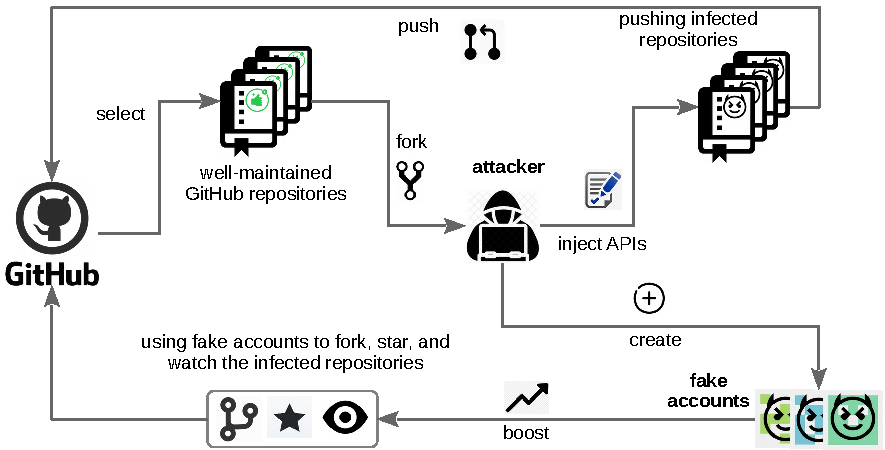
\includegraphics[width=0.450\linewidth]{figs/PushAttacks.pdf}
%	%\vspace{-.1cm}
%	\caption{Manipulating \GH to boost the visibility of malicious repositories~\cite{9678946}.} %Performing push attacks
%	\vspace{-.3cm}
%	\label{fig:PushAttacks}
%\end{figure}
%
%%Let us imagine a scenario in which one increases the popularity of malicious APIs\footnote{An API is considered as malicious if it causes fatal errors, no matter where it comes from, \ie either a legitimate or a fake library.} by planting them to OSS projects, as many as possible. 
%
%Figure~\ref{fig:PushAttacks} depicts a scenario, with which hostile users can follow to seed malicious repositories. First, attackers fork well-maintained repositories from \GH, \eg those that have good indicators with respect to the number of stars, forks, or watchers. Afterward, they inject projects with fake APIs, and then upload again to \GH. %In fact, malicious repositories are quite a phenomenon in \GH%are not scarce, but \emph{dime a dozen}
%%~\cite{Rokon2020SourceFinderFM}. 
%The visibility of a malicious API can be amplified by injecting it into a significant number of declarations for each training project. Moreover, to expose better the adversary repositories to search engines, attackers may create fake accounts to star, fork, and watch the malicious repositories.\footnote{Such manipulation has been recently revealed \url{https://zd.net/3bg3CK9}.} In fact, malicious repositories are quite a phenomenon, and many of them with malware apps have been detected in \GH \cite{Rokon2020SourceFinderFM}. %, and they might be only \emph{the tip of the iceberg}. %, waiting. 
%
%%There are precedents where thousands of repositories
%%===============================
%%Though RSSEs may choose %attempt to crawl training data from 
%%repositories considered to be \emph{credible}~\cite{NGUYEN2019110460}, \eg having a significant number of stars, forks, or watchers, unfortunately, this cannot help them completely evade toxic repositories. These metrics, however, can be falsified as attackers use fake accounts to star, fork, and watch the malicious repositories, making them appear more legitimate. Such a trick has been recently revealed, where several fake accounts are used to reciprocally endow their malicious repositories. %\footnote{\url{https://zd.net/3bg3CK9}} 
%%To our knowledge, research conducted to fight this type of abuse is still in its initial phase~\cite{10.1145/3357384.3357971}. %,Rokon2020SourceFinderFM
%%Thus, techniques to conduct attacks are known, and there are at least examples of fake repositories, albeit being created for other purposes rather than for attacking RSSE. 
%%===============================
%%Attacks may also impose different methods to hide their adversarial intent. Apart from wrapping malicious code in a single API call (see Section~\ref{sec:Example}), they might disguise it with a typosquatting name~\cite{10.1145/3463274.3463809}, \ie one that closely resembles a popular API. In this case, developers would adopt the disguised API/snippet without the least delay, once it is provided by the recommendation engine. 
%%===============================
%%increase their credibility/visibility, thus exposing them better to search engines
%%Then, based on the tool availability as well as the characteristics of the tools, 
%
%Following our main line of research in RSSEs~\cite{DBLP:journals/ese/RoccoRSNR21,NGUYEN2019110460,Nguyen:2019:FRS:3339505.3339636,10174041}, %in our recent work~\cite{9678946}, 
%by means of mixed methods research (\ie combining quantitative research and qualitative research), %mixed-method study %to a first empirical investigation 
%we shed light into the effects of adversarial machine learning in RSSEs~\cite{9678946}. Through a systematic literature review in premier software engineering venues, we found out that all of them deal with malware detection in Android apps, we did not find any work related to potential threats and implications of adversarial attacks to API RSSEs.
%%so far no existing study investigates the issue of adversarial attacks to API  recommender systems. % has not attracted attention from the research community. % major software engineering venues. 
%%First, through a literature analysis on 14 premier venues in software engineering, we show that there has been no work to study the issue of AML in RSSE. 
%%In summary, by thoroughly investigating the papers that match 
%%Using a set of keywords to filter out irrelevant studies, we realized that all of them deal with malware detection in Android apps. Instead, we did not find any work related to potential threats and implications of adversarial attacks to API RSSE.%recommender systems.
%
%
%Next, we performed an evaluation on three state-of-the-art API recommender systems, \ie \UM~\cite{Wang2013Mining}, PAM~\cite{Fowkes:2016:PPA:2950290.2950319}, and \FC~\cite{Nguyen:2019:FRS:3339505.3339636}, % 
%%underlining their risk of being manipulated by adversarial techniques. Then, we perform an empirical evaluation on three API recommenders 
%using repositories that have been injected with harmful APIs. 
%The results revealed a worrying outcome: by crafting input data to feed the systems, we succeeded in spoiling the recommendations, promoting fake/toxic API calls that can potentially harm the end users. %, \ie %. %Last but not least, we devise some possible countermeasures to cope with this type of manipulations. 
%%The results emerged from our quantitative analyses revealed that 
%%even with a small amount of artificial training data, the ratios that systems the fake APIs are always larger than 0. %, implying that clients are being provided with the fake APIs. 
%In particular, the results demonstrated that the use of PAM may be threatened by malicious attempts concealed in training data. Also for \FC, the seeded data has an adverse effect, \ie the tool is tricked into recommending to developers the toxic APIs, and source code. \UM is also not an exception, and it is prone to adversarial attacks, suggesting malicious APIs to developers.
%%We select three of them,  \ie \UM~\cite{Wang2013Mining}, PAM~\cite{Fowkes:2016:PPA:2950290.2950319}, and \FC~\cite{Nguyen:2019:FRS:3339505.3339636}. 
%%To evaluate the resilience of \UM, PAM, and \FC, we use a dataset containing Android apps' source code. %We focused on Android apps because they entail a typical scenario in which an infection can cause unwanted consequences such as data leaks.
%Altogether, we conclude that API recommender systems are likely to be exploited, and in this way they inadvertently become a \emph{trojan horse}, threatening the security of software systems. 
%
%The results of this work have been published in the proceedings of the ASE 2021 conference:% following paper:
%\vspace{-.1cm}
%\begin{itemize}
%	\item \small{\underline{Phuong T. Nguyen}, Claudio Di Sipio, Juri Di Rocco, Massimiliano Di Penta, Davide Di Ruscio ``\emph{Adversarial Attacks to API Recommender Systems: Time to Wake Up and Smell the Coffee?}'', in Proceedings of the 36th IEEE/ACM Int. Conf. on Automated Software Engineering (ASE 2021), DOI: \href{https://doi.org/10.1109/ASE51524.2021.9678946}{10.1109/ASE51524.2021.9678946}.}
%\end{itemize}
%
%\vspace{-.4cm}


%We have the following remarks:











%``\emph{}''




%\section{Goals} \label{sec:Goals}
%
%
%
%\begin{itemize}
%	\item a machine learning model to protect privacy in software engineering system.
%	\item users are reluctant to share their data.
%	\item machine learning models tailored to software engineering applications.
%\end{itemize}
%
%Fair and robust recommender systems for software engineering.

% an initial investigation of





%==========================================
%\subsection{Mining time series data in GitHub}
%
%In open-source software repositories, there exist time-series artifacts which are the result of the interaction between developers and hosting platforms, e.g., the evolution of a software project in GitHub over the course of time. %Similarly in MDE, models evolve during their lifecycle, resulting in the transformation and evolution of models. 
%Such type of data, once being properly mined, can provide developers/modelers with useful recommendations, helping them complete their tasks. 
%
%In this respect, I assume that the deployment of Machine Learning techniques such as Long Short-Term Memory recurrent neural networks (LSTM), or Encoder-Decoder LSTM allows us to mine the existing data, providing supports to developers. 
%%In this respect, ML techniques specialized
%%in dealing with sequential data are of great use, i.e., 
%These algorithms are able to learn from time series data to perform predictions for unknown sequences of events. Some initial attempts have already been made following this paradigm, achieving a promising performance.
%%For instance, Burgueño et al. [121] proposed an automatic approach to model trans-
%%formations built on top of an LSTM neural network. 
%Once trained, the systems can
%automatically transform an input model into the corresponding output without needing any transformation-specific code. Furthermore, I anticipate that the application of cutting-edge neural networks %, %such as Encoder-Decoder, or Transformer, 
%can help tackle various issues, including model transformation and model evolution, further boosting the prediction capability.
%==========================================


\section{Methodology}
\label{sec:Methodology}

%\subsection{Introduction}







%===================================================The aim of this paper===============================================
%We first provide an overview of state-of-the-art API and third-party library recommenders, discussing  how they could be potentially affected by AML.

%Through a literature search from premier venues in Software Engineering for adversarial techniques, I show that there are considerably evident threats to RSSE. 
%Then, we perform a preliminary examination of two existing systems for recommending third-party libraries. The experimental results reveal a worrying outcome: by a simple manipulation, we can seamlessly spoil the final recommendations, putting software clients at risk.

%In this section, we present the proposed approach.

%The prospective work is not a fresh %completely new 
%start, but a continuation of our current research presented in Section~\ref{sec:CurrentResults}. %Our focus is to find methods to defuse popularity bias, and deal with adversarial attacks. 


%The research aims to contribute to the resilience and trustworthiness of recommender systems used in software engineering contexts, ultimately safeguarding users and valuable software assets. 
Figure~\ref{fig:SystemArchitecture} depicts the architecture with the proposed module being printed in the cyan color, which can be independently assembled to any existing recomender systems, %. The first module is used to detect and eliminate adversarial intents disguised in the training data, meanwhile, the second module is 
being padded right before the interface to developers to defuse popularity bias.
This section presents our proposed approach to fill the research gap introduced in Section~\ref{sec:Introduction}. %, before presenting the results.



%\subsection{Adversarial attacks}

%\section{Project overview}

%\section{Background}
% \cite{Dagenais:2010:MNS:1806799.1806842} (often at a short time)

%Deep learning techniques exploit multiple layers to better capture features from an input and.
%Deep Neural Networks architectures are designed 
% where every single layer only receives a connection from previous and provides connections only to the next layer in the hidden part
%The implementation of Deep Neural Network (DNN) is basically a discriminatively trained model that uses the standard back-propagation algorithm and sigmoid or ReLU as activation functions. 
%assigns more weights to the previous data points of sequence. Therefore, this technique is 
%can be used for text mining and classification. 
%considers the information of previous nodes in a very sophisticated method which 
%Deep learning is a technique that allows computational models composed of multiple processing layers 

%In the domain of Mining Software Repositories (MSR), 
%the ultimate aim is to discover serendipitous relationships among open source software projects by analyzing the rich data available in software repositories. In software repositories, the volume of data grows exponentially and turns to be increasingly inconsistent over the course of time. At the expense of the data model, data accessing and processing appears to be a daunting task. This makes the cost for maintaining information integrity become prohibitive. The requirement of knowledge sharing and interoperability necessitates an adequate modeling of diverse software artifacts, e.g., issue tracker, version tracker. Given the heterogeneity and constant changes of the underlying distributed data in MSR, the utilization of XML and databases is not sufficient for fulfilling the above mentioned requirements. Furthermore, the lack of a common format in software repositories makes it difficult to integrate data from various sources to produce recommendations as well as to forecast project evolution. To this end, a uniform knowledge base that facilitates data representation and integration is of highly importance. The knowledge base is expected to render possible innovative features and enable the discovery of useful or interesting relationships by chance. Based on this representation, it is then possible to detect project incompatibilities and to identify complementary and competing projects. 

%I propose conducting a prospective research which is going to be based on three core research theme: \emph{Mining OSS Repositories}, \emph{Recommender Systems}, and \emph{Deep Learning}. 
%In this sense, DNN exploit the standard back-propagation algorithm and sigmoid or a rectified linear unit (ReLU) as the activation function. Several deep neural network architectures have been proposed to increase both prediction accuracy and efficiency. 
%The ability to . 
%and from existing data by 
%To integrate various types of recommendations. 

%Conventional neural networks connect all the neurons of a layer to the next layer, and the number of weights increases over the number of layers. 

%For building and 
% the capability
%into 
%First, it is necessary to provide developers with instant recommendations. The re that best fit their needs. 
%This is done 
%assign more weights to the previous data points of sequence. An RNN 

%===================================
%An LCD platform needs to be equipped with built-in modules offering various functionalities, which can be instantly embedded whenever developers drag and drop them into their working panel. Such modules are provided by mining OSS repositories to integrate different types of recommendations. To this end, I plan to investigate and deploy suitable recommender systems to supply different artifacts, \eg source code, API usage patterns, third-party libraries. Furthermore, I am going to study the feasibility of applying DNNs to generate recommendations, \eg source code classification, software size estimation, automatic software repair, API sequences, to name a few. For instance, Recurrent Neural Networks (RNNs) are a family of neural network architectures that allow for better semantic analysis of the structures in a dataset, thereby being highly suitable for the classification of textual and sequential data. RNNs can be used to classify software systems by means of source code, or to classify API documentation. Still, the identification of suitable DNNs for mining OSS repositories is dependent on a more detailed investigation. 

%clustering open source software projects 
%In this sense, I am going to investigate in detail the suitability of.

%\vspace{-.3cm}

\begin{figure}[h!]
	\centering
	%	\vspace{-.2cm}
	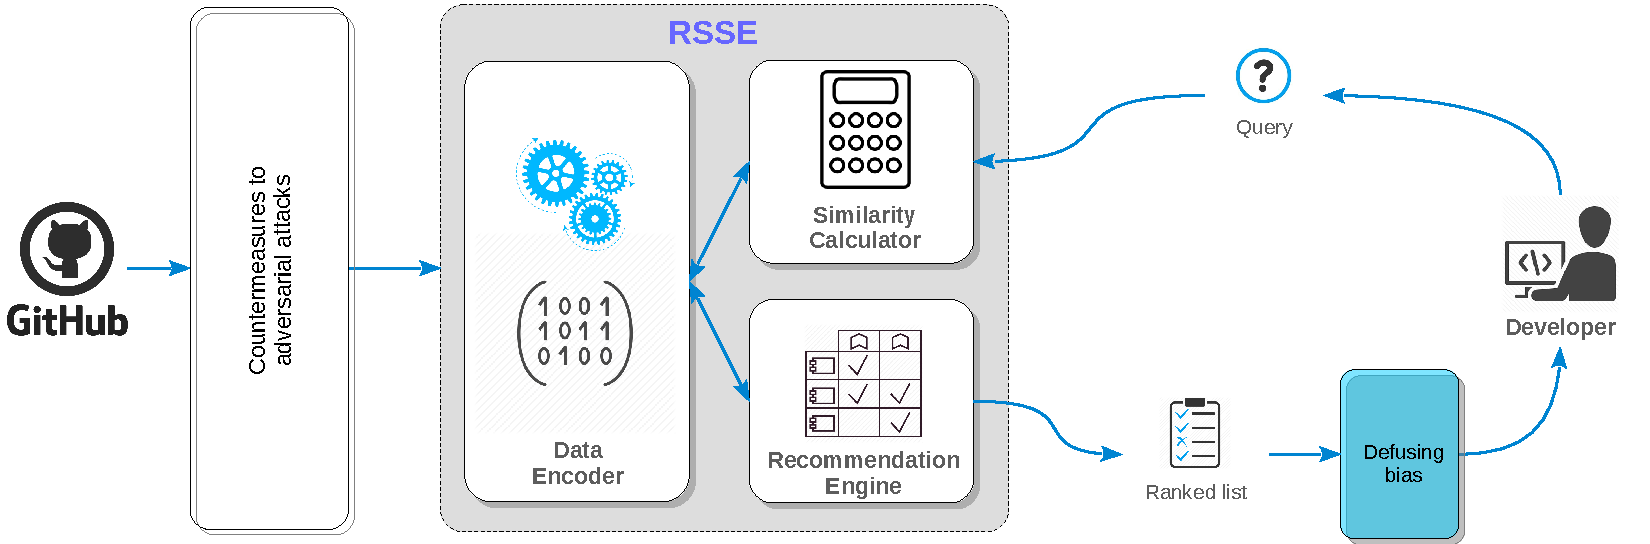
\includegraphics[width=0.60\columnwidth]{figs/SystemArchitecture.pdf}
	\vspace{-.2cm}
	\caption{The proposed architecture.}
	\vspace{-.4cm}
	\label{fig:SystemArchitecture}
\end{figure}


%=================================
%\begin{figure}[h!]
%	\centering
%	%	\vspace{-.2cm}
%	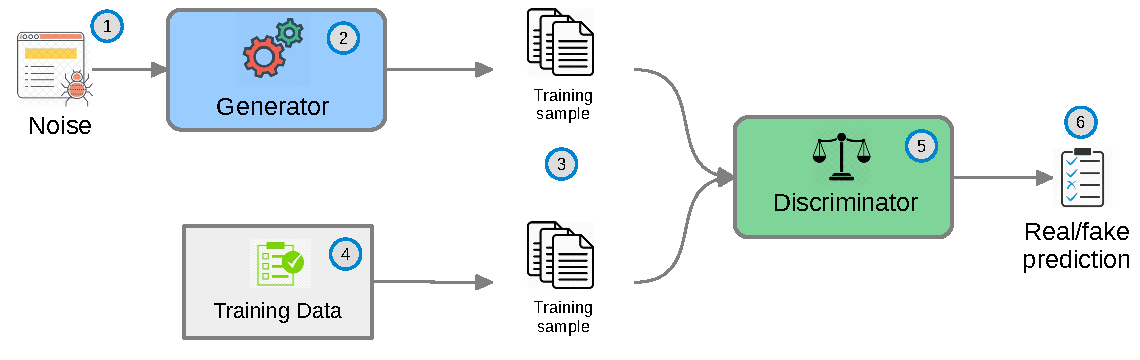
\includegraphics[width=0.60\columnwidth]{figs/GAN.pdf}
%	\vspace{-.2cm}
%	\caption{Architecture of a Generative Adversarial Network~\cite{DBLP:journals/csur/WangSW21}.}
%	%	\vspace{-.3cm}
%	\label{fig:GAN}
%\end{figure}
%=================================






\subsection{Research objectives}




%	\item a machine learning model to protect privacy in software engineering systems.
%	\item Users are reluctant to share their data.
%	\item Machine learning models tailored to software engineering applications.

%Within the project funded by Sony, 
%In particular, 

%We are going to conceptualize suitable techniques for building %address the related issues 
%fair and robust recommender systems for Software Engineering by 

%To be concrete, 
%Correspondingly, 
Within the funded project, we are going to answer the following research questions.

%The present paper makes the following contributions: 
%\begin{itemize}
%	%	\noindent
%	\item[--] A discussion on the possible adversarial attacks to state-of-the-art RSSE for third-party libraries and API calls; 
%	\item[--] A preliminary evaluation on two library recommender systems to perturb their recommendations.
%\end{itemize}

\begin{itemize}

	\item[--] \textbf{RQ}: ``\emph{How can we make RSSEs less biased towards popular items, while still preserving accuracy?}'' We plan to develop novel methods to defuse popularity bias. Existing mechanisms conceived for other domains might not work well for recommender systems for software engineering, as we showed in our recent work~\cite{10174041}. We anticipate that Reinforcement Learning~\cite{DBLP:books/lib/SuttonB98} can be applied to improve re-ranking techniques, taking into consideration the similarity between projects when a rare library needs to be moved up in the ranked list. %the libraries that need to re-ranked, and the ones that contain.	
	
%	\item[--] \textbf{RQ2}: ``\emph{How can we defend RSSEs against adversarial attacks?}'' Given the existing threats, it is necessary to conceive effective countermeasures that can ward off attacks tailored to RSSE. This is done by studying learning algorithms being aware of adversarial attacks and seize them. Moreover, adversarial attempts should be turned into features for the 
%	training process, \ie RSSEs should not only learn from useful patterns, but also be able to learn how to avoid hostile patterns.
\end{itemize}

%, while allowing 
%Our work reveals that software engineering research has not properly dealt with popularity bias in TPL RSSEs, triggering the need for effective counteracting mechanisms. %Looking at other domains, 
%we see that there are three major methods to combat bias in general, \ie the pre-processing, in-processing, and post-processing paradigms~\cite{doi:10.1089/big.2016.0048}. We assume that they can also be adopted in Software Engineering for the same purpose, as it was also advocated by Chakraborty \etal \cite{ChakrabortyM0M20}, though not directly for RSSEs. %Also, as it can be seen from Section~\ref{sec:Results}, He \etal~\cite{9043686} conceived 
%\LS~\cite{9043686} is the very first TPL RSSE to mitigate the abundance of highly frequent libraries, following the \emph{in-processing} approach. \LS attempts to neutralize the bias caused by the popularity of TPLs using an adaptive weighting mechanism. However, while it can diversify the recommendations, \LS suffers from a low accuracy (see RQ2 in Section~\ref{sec:RQ2}). This implies that there is still room for improvement, \ie conceiving more effective in-processing techniques for RSSEs.


To answer the research question, correspondingly we divide the tasks into two tasks, namely \textbf{T1} and \textbf{T2} (see Figure~\ref{fig:SystemArchitecture}), and they are explained in the succeeding subsections.
%\vspace{-.4cm}


\subsection{Defusing popularity bias}

%Our work~\cite{10174041} reveals that the issue of popularity bias in RSSEs has not attracted attention from the research community, triggering the need for effective counteracting mechanisms. 
Looking to other domains, we see that there are three major methods to defuse bias in general, \ie the pre-processing, in-processing, and post-processing paradigms~\cite{doi:10.1089/big.2016.0048}. We suppose that these can also be adopted in software engineering for the same purpose. %as it was also advocated by Chakraborty \etal \cite{ChakrabortyM0M20}, though not directly for RSSEs. 
We are going to perform the following tasks:

\begin{itemize}
	\item \textbf{T1: Re-implementation of existing re-ranking mechanisms.} In our recent work~\cite{10174041}, we applied xQuAD \cite{10.1145/1772690.1772780} %--an algorithm for diversifying Web search results, 
%	and the technique allowed us 
	to improve diversity in the recommendations. %Nevertheless, such the improvement is marginal, and there exists a light setback in accuracy. 
	We plan to investigate and re-implement other %re-ranking 
	techniques, with the aim of finding suitable mechanisms to be adopted for RSSEs. Another possible candidate is PFAR~\cite{DBLP:journals/corr/abs-1809-02921}, a practical approach conceived to allow items to have a fair chance of being recommended. We will considered also personalized ranking~\cite{DBLP:conf/flairs/AbdollahpouriBM19}, which promotes unpopular items in the ranked list, while maintaining a trade off between fairness and accuracy. Once re-implemented, these techniques can be used as baselines for comparison with our proposed approach presented in \textbf{T2}. %as well as to i%Thus, it is necessary. 
%, \eg the frequency of occurrences may. %, \eg r.
%\emph{Pre-processing} techniques can also be useful for TPL RSSEs, \eg by considering factors related to peculiar, solution-specific aspects of a project that, as pointed out in Section \ref{sec:Background} are neglected, and that would help reward certain libraries. From RQ1, we see that no approach specifically employs pre-processing to cope with popularity bias in RSSEs.
	\item \textbf{T2: Reinforcement learning for reducing bias.} Existing re-ranking algorithms such as xQuAD~\cite{10.1145/1772690.1772780} %rearrange the recommendation lists, aiming 
	attempt to reduce the number of popular items, as well as to increase the number of unpopular (but useful) ones in the results. However, our empirical evaluation on two recommender systems showed that while introducing diversity in the recommendation results, it also introduces a setback in the prediction accuracy. Our findings suggest that %Software Engineering 
	further research should be conducted to propose effective countermeasures. We suppose that it is crucial to consider %further improve it by considering 
	additional factors, \eg the degree of specificity (to certain solutions) of a library, when it comes to providing recommendation. Thus, we will deploy Reinforcement Learning to implement effective post-processing techniques to defuse popularity bias, aiming to improve diversity in the recommendations, while keeping a reasonable prediction accuracy. % without touching the internal design of the considered systems.
	% ...%The technique is built 
%Starting from an initial ranked list $R$, we look for the long-tail items in the list, and promote them to upper positions to yield a new list $S$. %We call %$R$ as the list provided by a recommender, and 
%$S$ is initially set to $\varnothing$, and iteratively populated by enrolling new items using the following formula.
%	\item The result of this workpackage is Deliverable \textbf{D1}: ``\emph{Defusing popularity bias with reinforcement learning}.''
\end{itemize}
\vspace{-.4cm}


%\subsection{WP2: Generating malicious data; Adversarial training}
%
%%Generative Adversarial Networks
% 
% \begin{itemize}
%	\item[--] \textbf{T2.1: Generating fake data with GANs.} %\textbf{RQ2}: ``\emph{Can GAN cause threats to third-party library and APIs recommender systems?}'' 
%%We plan to study the threats that cause harm or danger to RSSE suggesting third-party libraries and API function calls. %These two types of recommendations have been selected as they are representative scenarios in which \emph{(i)} the recommendation is learned from OSS repositories; and \emph{(ii)} the outcome of a malicious recommendation, \eg the usage of a library or an API, can cause troubles to end-users.%result in severe security holes.%~\cite{10.1145/2976749.2978333}.
%To defend a system against attacks, it is necessary to be knowledgeable of various types of adversary activities~\cite{4216981}, which generate perturbations to deceive and disrupt systems by %causing a malfunction, 
%compromising their recommendation capabilities. 
%%A main way to achieve this is to feed systems with malicious data~\cite{DDM20a}.
%The ultimate aim of these attacks is to manipulate target items, thus creating  either a negative or positive influence on the final recommendations~\cite{10.1007/s10462-012-9364-9}, depending on the attacker's 
%intention. %For instance, in image classification, an attacker crafts an input image by adding non-random noise in a way that it will be imperceptible to ML models, whilst still being properly recognized by 
%%humans~\cite{conf/cvpr/NguyenYC15}. As an example, a panda was recognized as a ribbon by cutting-edge deep neural networks once the input image had been padded with noise, meanwhile humans still correctly perceived the panda from the forged image~\cite{DBLP:journals/corr/GoodfellowSS14}.
%Generative Adversarial Networks \cite{10.5555/2969033.2969125} (GANs) have been widely used in image processing to produce crafted images, which resemble real ones. %are a very popular class of deep generative models which have shown some incredible results in generating images. 
%GANs consist of two main components, \ie Generator and Discriminator. Generator is a deep neural network and accepts as input both real training data and crafted data, \ie noise. %is trained to take a random input $z$.
%%The idea behind GANs is to train two networks simultaneously. 
%%Firstly, a generator network, which we can train to take a random input (often called  z) and produce a sample from some distribution, in this case, the distribution of 28 $\times$ 28 grayscale clothing images. 
%Discriminator is also a deep neural network and it learns to distinguish the real training data from the crated data, to provide the final prediction. In other words, Generator is trained with real and forged data to trick Discriminator, which in turns attempts to avoid being tricked by learning from real training data.
%According to our investigation, GANs can also be exploited to generate fake training data to feed RSSEs. %This section briefly recalls the main technical details of GANs.\footnote{The background of GANs as well as the corresponding notions originate from \url{https://bit.ly/3hizVtf}} %Deep neural networks have been exploited to generate perturbations.  
%We suppose that GANs can be used to produce crated training OSS projects to compromise RSSEs. In this respect, it is necessary to perform a detailed investigation on this topic, as well as to find effective countermeasures that can deal with this type of adversarial attempts.

%	\item[--] \textbf{T2.2: Anomaly detection and adversarial training.} To mitigate the impact of ill intents to recommender systems, anomaly detection techniques can be considered as a viable strategy. This involves identifying malicious API patterns before they are recommended to developers. For instance, a statistical process control strategy~\cite{10.1145/1097047.1097061}, has proven effective in recognizing suspicious items by assessing two critical parameters: the distribution density of items and their average ratings. For RSSEs, detecting anomalies corresponds to the distribution patterns of APIs within software projects and declarations. %However, it is imperative to approach this task with care to minimize the risk of false positives and false negatives. 
%API distributions can span a wide spectrum, covering not only extremely popular APIs but also rare and less common ones. Therefore, relying solely on radical patterns, such as those that are excessively popular or exceedingly rare, may not guarantee successful discrimination in all cases. A more tailored approach involves the detection of malicious and benign API sequences by monitoring a specific set of third-party libraries with supervised classifiers~\cite{10.1109/COMPSAC.2015.241}. While this approach holds promise, it does not come without limitations, \ie it may perform well in detecting malicious sequences comprised of APIs from a predefined set of libraries, but may not be universally applicable to patterns containing only a few APIs sourced from less popular libraries. %, warranting further exploration and refinement.
%	\item[--] The results of this workpackage is Deliverable \textbf{D2}: Dealing with fake data using adversarial training.
%
%\end{itemize}


%========================
%Figure~\ref{fig:GAN} illustrates a GAN which consists of two main components, namely Generator and Discriminator. Generator \circled{2} is a deep neural network and accepts as input both real training data \circled{4} and crafted data \circled{1}, \ie noise. %is trained to take a random input $z$.
%%The idea behind GANs is to train two networks simultaneously. 
%%Firstly, a generator network, which we can train to take a random input (often called  z) and produce a sample from some distribution, in this case, the distribution of 28 $\times$ 28 grayscale clothing images. 
%Discriminator \circled{5} is also a deep neural network and it learns to distinguish the real training data from the crated data, to provide the final prediction \circled{6}. In other words, Generator is trained with real and forged data to trick Discriminator, which in turns attempts to avoid being tricked by learning from real training data. %This process is described in the following diagram:
%
%
%%The main idea is to train the generator with and discriminator, by minimizing the. 
%%(one that makes the fewest mistakes possible) 
%% Of course, in practice, we do not necessarily have an optimal discriminator, and so we end up with some approximation of the JSD.
%%Let's take a closer look at what the JSD is and how it is approximated.
%%We can, and will in just a moment, prove that 
%%https://colab.research.google.com/github/khipu-ai/practicals-2019/blob/master/3b_generative_models.ipynb#scrollTo=5f0u8t0K5FOk
%
%In this context, Discriminator plays the role of a loss/error function to train Generator. %by approximating the Jensen-Shannon divergence (JSD). 
%Using Discriminator to train Generator boils down to minimizing the JS-divergence between the distributions of the generated and real data. The final aim is to minimize the loss, which is defined using the following formula \cite{10.5555/2969033.2969125}:
%
%%In this respect, Jensen-Shannon Divergence (JSD) is used to measure the similarity between two probability distributions. 
%
%\begin{equation} \label{eqn:loss1}
%	E_{x\sim p_{d}(x)}\left [ log D^{*}(x)\right ] + E_{z\sim p_{z}(z)}\left [ log(1-D^{*}(G(z)))\right ]
%\end{equation}
%
%%from which we draw samples to pass through our generator
%%\vspace{-.2cm}
%$D^{*}(x)$ is defined as follows:
%\begin{equation} \label{eqn:D}
%	D^{*}(x) = \frac{p_{d}(x)}{p_{d}(x)+p_{g}(x)}
%\end{equation}
%
%where $p_{d}(x)$ is the distribution of the training data, and $p_{z}(x)$  is the distribution of the noise. 
%
%The first component, \ie $E_{x\sim p_{d}(x)}\left [ log D^{*}(x)\right ]$ corresponds to attempts to recognize real data better, while the second component, \ie $E_{z\sim p_{z}(z)}\left[ log(1-D^{*}(G(z)))\right ]$ means that the engine can spot fake data better.
%========================





%By substituting Eq.~\ref{eqn:D} into Eq.~\ref{eqn:loss1}, we get the following equation.
%\begin{equation}
%E_{x\sim p_{d}(x)\left [ log D^{*}(x)\right ]} + E_{z\sim p_{z}(z)\left [ log(1-D^{*}(G(z)))\right ]}
%\end{equation}
%\vspace{.2cm}





%	\item  









%
%\subsection{WP2: Countermeasures to adversarial attacks}
%
%
%To equip RSSEs with robust defense mechanisms against malicious endeavors, we are committed to developing innovative techniques to identify and thwart malicious APIs. Additionally, we acknowledge the significance of adversarial training, \ie training machine learning models on manipulated data to enable them to discern adversarial intent from benign ones. %To this end, 
%Our research will focus on the following key tasks:%key aspects:
%
%%To equip RSSEs with effective mechanisms to defend against hostile attempts, we will develop %countermeasures %. We intend to develop defense mechanisms from the following two perspectives: \emph{(i)} internal view, \ie design of recommender systems; and \emph{(ii)} external view, 
%%techniques to %detect and protect against hostile attempts, %. Concerning the former, we study counteractions conceived for generic recommender systems in the hope of customizing them for RSSE. With the latter, 
%%recognize and seize malicious APIs. Moreover, we also consider adversarial training, \ie training a machine learning model with manipulated data, so as allowing it to learn how to distinguish bad intents from the good ones. In particular, our proposal will be focused on the following aspects:%techniques:
%
%%===========================https://bkai.ai/seminar-adversarial-learning-foundations-and-applications/===========================
%%Adversarial robustness aims to improve the robust accuracy of ML models on adversarial data, which can be achieved by adversarial training (AT). Specifically, AT has two purposes: (1) correctly classify the data (the same as ST) and (2) ensure no data fall nearby the decision boundaries (different from ST). Given that the test data may be adversarial, AT carefully simulates some adversarial attacks during training. Thus, the model has already seen many adversarial training data in the past with the purpose of generalizing to adversarial test data in the wild. 
%%===========================
%%In the following, we discuss possible 
%
%% and protect RSSE. %API recommender systems.%anomaly detection techniques that can be used for API recommenders.
%%Countering adversarial attacks through a
%
%
%\begin{itemize}
%	\item \textbf{T2.1: Mitigating the impact of manipulated projects.} Utilizing model-based algorithms offers a valuable approach for addressing the influence of manipulated profiles within recommender systems, particularly in the context of open-source software (OSS) projects~\cite{4216981}. These algorithms excel in the task of categorizing similar profiles, effectively grouping OSS projects into distinct segments. While these techniques may not provide absolute immunity against malicious projects, their primary goal is to diminish the prevalence of projects exhibiting abnormal behaviors. Such projects should not be categorized as similar to any active or legitimate projects currently under development. This methodology allows us to significantly reduce the likelihood of %recommender 
%	systems selecting and incorporating deceptive or spurious data, thus defending them against from potential attacks. Moreover, this approach can be applied to improve the security of RSSEs relying on similarity, %or collaborative-filtering techniques, 
%	\eg UP-Miner \cite{Wang2013Mining}, MUSE \cite{Moreno:2015:IUT:2818754.2818860}, FOCUS~\cite{Nguyen:2019:FRS:3339505.3339636}, or CodeKernel \cite{DBLP:conf/kbse/Gu0019}. %However, it is worth noting that implementing this method necessitates the thorough redesign of the foundational building blocks of these systems, making it a complex endeavor that may require substantial effort and resources.% to execute effectively.
%
%%	\item \textbf{T2.2: Enhancing resilience through profile classification.} Profile classification can be an effective mechanism in fortifying the resilience of RSSEs against malicious attacks~\cite{10.1145/1097047.1097061}. The process begins by constructing a training dataset that encompasses both authentic projects and synthetic projects generated according to a predefined attack model. To streamline the dataset, attribute-reduction techniques can be applied, reducing the number of features required for representation. Following dataset preparation, supervised classifiers are trained on the refined dataset. The ultimate objective is to distinguish between genuine and synthetic projects, effectively detecting instances where malicious data has been inserted. The efficacy of this technique is enhanced given that an ample volume of training data is available, covering diverse approaches to populating synthetic (fake) projects. We postulate that a multifaceted approach, %implementation of a hybrid security model, 
%%	which aggregates internal and external perspectives, holds significant promise in boosting the robustness and resilience of RSSE against adversarial attacks. Internal countermeasures enable RSSEs to preemptively sidestep falsified data sources, while external-view defense mechanisms facilitate the detection of concealed malicious intent within API patterns before recommending them to developers. %This multifaceted approach serves as a comprehensive shield against potential threats to RSSE integrity.
%	
%	\item \textbf{T2.2: Anomaly detection and adversarial training.} To mitigate the impact of ill intents to recommender systems, anomaly detection techniques can be considered as a viable strategy. This involves identifying malicious API patterns before they are recommended to developers. For instance, a statistical process control strategy~\cite{10.1145/1097047.1097061}, has proven effective in recognizing suspicious items by assessing two critical parameters: the distribution density of items and their average ratings. For RSSEs, detecting anomalies corresponds to the distribution patterns of APIs within software projects and declarations. %However, it is imperative to approach this task with care to minimize the risk of false positives and false negatives. 
%	API distributions can span a wide spectrum, covering not only extremely popular APIs but also rare and less common ones. Therefore, relying solely on radical patterns, such as those that are excessively popular or exceedingly rare, may not guarantee successful discrimination in all cases. A more tailored approach involves the detection of malicious and benign API sequences by monitoring a specific set of third-party libraries with supervised classifiers~\cite{10.1109/COMPSAC.2015.241}. %While this approach holds promise, it does not come without limitations, \ie it may perform well in detecting malicious sequences comprised of APIs from a predefined set of libraries, but may not be universally applicable to patterns containing only a few APIs sourced from less popular libraries. %, warranting further exploration and refinement.
%	\item The result of this workpackage is Deliverables \textbf{D2}: ``\emph{Defending RSSEs against adversarial attacks,}'' and \textbf{D3}: ``\emph{A holistic approach to fairness and robustness of RSSEs}.''%Defending RSSEs against adversarial attacks. %Dealing with adve using adversarial training.
%		
%\end{itemize}
%\vspace{-.4cm}
%%``\emph{}.''
	
%	\item \textbf{Minimizing the effect of manipulated profiles.} Model-based algorithms are of great use as they can be applied to cluster similar profiles (OSS projects) into \emph{aggregate segments}~\cite{mobasher_attacks_2007}. Though these techniques cannot entirely isolate malicious projects, this aims to lessen the prevalence of projects with abnormal behaviors, \ie they will not be seen as similar to any active projects, \ie the ones under development. In this way, such a method reduces the possibility that RSSE select and incorporate bogus data, thereby avoiding attacks. The method can be applied to defend RSSE that work based on a similarity or collaborative-filtering technique, such as UP-Miner \cite{Wang2013Mining}, MUSE \cite{Moreno:2015:IUT:2818754.2818860}, FOCUS~\cite{Nguyen:2019:FRS:3339505.3339636}, or CodeKernel \cite{DBLP:conf/kbse/Gu0019}. Nevertheless, it requires the redesign of the whole systems' underpinning building blocks, and thus, it is not easy to conduct.  %Furthermore, it may not be applicable to other systems, such as MUSE, or.
%	\item Adversarial attacks can be counteracted using \textbf{anomaly detection techniques}, \ie recognizing malicious API patterns before they are recommended to developers. %There have been approaches conceived to detect malicious API sequences. 
%	For instance, a statistical process control strategy~\cite{mobasher_attacks_2007} has been used to identify suspicious items by examining two parameters, namely items' distribution density and average ratings. By referring to RSSE, we can think of detecting anomalies from the distributions of APIs in projects and declarations. This, however, necessitates careful analyses to avoid false positives and false negatives. %As shown in Section~\ref{sec:rq2-design}, 
%	The distributions of APIs may span in a wide range, \ie there are not only extremely popular APIs but also rare ones. Thus, being based on a radical pattern, \eg a too popular or too rare one, the detection of malicious APIs may not succeed in every case. A more tailored approach is to tell malicious/benign API sequences apart by monitoring a certain set of third-party libraries using supervised classifiers~\cite{10.1109/COMPSAC.2015.241}. Such an approach, however, has its limitation as follows. Though it can detect malicious sequences consisting of APIs from a specific set of libraries, it may not be applicable to patterns with a few APIs coming from a less popular library.
%	\item \textbf{Profile classification} can also help increase the resilience of RSSE against malicious attacks~\cite{10.1145/1097047.1097061}. First, it is necessary to build a training set consisting of both authentic projects and fake projects that are generated following an attack model. Attribute-reduction techniques may be used to reduce the number of features needed to represent the dataset. Afterward, supervised classifiers are trained on the resulting dataset to classify real and fake projects, aiming to detect the injection of malicious data. This technique works more effectively when we have enough training data by taking into consideration different ways of populating fake projects. In conclusion, we believe that a hybrid security model, consisting of countermeasures pertaining to both an internal (design) and external view, is likely to contribute to the robustness and resilience of RSSE towards adversarial attacks. While internal countermeasures allow RSSE to avoid falsified or suspicious data sources, defense mechanisms based on external view help RSSE detect malicious intent hidden in API patterns before recommending them to developers.%, RSSE may check for its eligibility.

%\UM~\cite{Wang2013Mining}, PAM~\cite{Fowkes:2016:PPA:2950290.2950319}, and \FC~\cite{Nguyen:2019:FRS:3339505.3339636}



%I am going to conduct an evaluation on two library recommender systems to perturb their recommendations. 








\section{Expected results and plans}
\label{sec:Results}
%The funded project is expected to . 

The proposed research on fairness %and addressing adversarial attacks 
in recommender systems for software engineering has the potential to yield significant outcomes, %. %, which can have far-reaching effects on both academia and industry. 
%Our proposed approach %extend beyond mere security enhancements, and 
%has the potential to 
positively impacting the software engineering field, artificial intelligence, user privacy, and the broader software industry. 
%The findings and defense mechanisms developed in this research will be disseminated through academic publications and presentations, contributing to the body of knowledge in software engineering. % security and adversarial machine learning. %This section elaborates on the implications of our work, as well as the prospective publications. % as follows.
\vspace{-.4cm}
\subsection{Implications}

%These implications are outlined below:


%The proposed research on fairness in recommender systems for software engineering has the potential to yield several significant implications and outcomes, which can benefit both academia and industry. These implications are outlined below:

%The implications of 


%=========================

\begin{itemize}
	\item \textbf{Enhancing user trust and satisfaction.} By mitigating bias and promoting fairness in recommender systems, our approach aims to enhance user trust and satisfaction with software engineering platforms. %This will help to improve user engagement and loyalty. %Enhanced System Security: 
	%With the conceived methods to defend RSSEs against adversarial attacks, our research can enhance the security and robustness of recommender systems used in software engineering platforms. This is crucial for safeguarding sensitive data and ensuring system integrity. %Preservation of User Trust: 
	As users rely on recommendations to make critical decisions in software engineering, our research helps to preserve user trust by ensuring that recommendations remain trustworthy.

	\item \textbf{Improving system performance.} Fairness-aware recommender systems are likely to generate recommendations that are not only unbiased but also more accurate and relevant to users. This improvement in recommendation quality can positively impact the overall performance of software engineering platforms. %The ability to thwart adversarial attacks can help maintain the reliability of recommender systems, ensuring that users receive dependable recommendations even in the presence of malicious actors.

%	\item \textbf{Ethical and responsible AI development.} Addressing fairness issues in recommender systems aligns with the principles of ethical and responsible AI development. Our research contributes to the responsible use of AI in software engineering by reducing potential biases and discrimination. %Protection of User Privacy: 
%	Addressing adversarial attacks can lead to improved protection of user privacy within recommender systems. This is particularly important in software engineering, where proprietary and confidential information is frequently handled.
 
%%	\item \textbf{Industry Adoption.} 
%	\item \textbf{Applicability.} 
%%	The recent years witness a proliferation of Large Language Models (LLMs). 
%	The potential of Large Language Models (LLMs) in Software Engineering has been considered to be enoumous~\cite{10109345}. %Among others, ... still containing bias. 
%	Nevertheless, such models are trained with a lot of data coming from different sources, and among other issues, bias and adversarial attacks. LLMs still rely on prompt tuning to function, \ie to be tailored for a specific purpose, they need to be fine tuned with proper data. In this respect, the techniques conceived from this research project can come in handy, defusing bias, and detecting adversarial intents in the training data. % can be used.
%	For industry, our approach and research outcomes can be adopted by software engineering companies, and integrated into their recommender systems. This will foster a culture of fairness and inclusivity in the industry, as well as the attitude towards the protection of users from adversarial threats. %Our defense mechanisms and research outcomes can be adopted by software engineering companies, enhancing the security of their recommender systems and protecting their users from adversarial threats.


	
	\item \textbf{Applicability.} The potential of Large Language Models (LLMs) in software engineering has been recently acknowledged~\cite{10109345}. However, these models are trained on vast and diverse datasets, which can introduce biases. Additionally, LLMs often require prompt tuning to tailor them to specific purposes, necessitating fine-tuning with relevant data. 
	In this context, the techniques developed in this research project offer practical solutions by mitigating biases within training data for LLMs. %For the software engineering industry, our approach and research outcomes hold substantial promise, \ie they can be readily adopted by software companies, seamlessly integrated into their recommender systems. This adoption promotes a culture of fairness and inclusivity within the industry. %Furthermore, it underscores a commitment to safeguarding users from potential adversarial threats. 
	%By addressing these critical issues, our research significantly enhances the applicability of Large Language Models in software engineering, making them more robust, ethical, and aligned with industry standards.
	
	\item \textbf{Educational impact.} The ethical implications of AI, including bias mitigation and adversarial counteraction, have gained significant attention in recent years. Our research offers an opportunity to educate future AI professionals about the importance of ethical considerations when developing AI-based systems. It can be integrated into AI ethics courses to promote responsible AI development. %Essentially, the developed fairness-aware attack-proof recommender systems can serve as learning materials, % for software engineering and AI courses, %promoting responsible AI development among students, %future professionals, %. The conceived defense strategies against adversarial attacks can be used as educational material for software engineering and cybersecurity courses, 
	%providing students with the knowledge and skills to protect recommender systems.
	
%	\item \textbf{Social impact.} After the devastating earthquake in L'Aquila in 2009,\footnote{L'Aquila Earthquake 2009 \url{https://www.internetgeography.net/topics/laquila-earthquake-2009/}} several efforts have been made to revitalize the city. Among others, investment in education and research is the key contributing factor, making the city become accessible to more people.
%	%The foundation of the Gran Sasso Science Institute. 
%	At the University of L'Aquila, we are committed to do cutting-edge research in various disciplines, including software engineering. 
%%	We will contribute to. 
%	Having a project funded by Sony will allow us %the University of L'Aquila 
%	to attract more external/foreign researchers to come to, and work in L'Aquila. More importantly, doing pioneering research %in the fairness 
%	in software engineering will help the university and thus, the city, increase their ranking and visibility. % of the University, as well as the city.
	
	
%	This will help  

%	\item \textbf{Interdisciplinary Collaboration.} This research may also encourage interdisciplinary collaboration between software engineers, data scientists, ethicists, and legal experts, fostering a holistic approach to addressing fairness issues, and adversarial challenges.
\end{itemize}
%=========================
\vspace{-.4cm}



%Maintenance of System Reliability: The ability to thwart adversarial attacks can help maintain the reliability of recommender systems, ensuring that users receive dependable recommendations even in the presence of malicious actors.

%Reduced Economic Losses: Adversarial attacks can have significant economic consequences, including financial losses due to system breaches and fraudulent activities. Our research can contribute to reducing these economic losses.

%Legal and Regulatory Compliance: In many jurisdictions, data protection regulations require organizations to implement security measures to protect user data. Our research can assist software engineering platforms in complying with these regulations.

%Knowledge Dissemination: The findings and defense mechanisms developed in this research will be disseminated through academic publications and presentations, contributing to the body of knowledge in software engineering security and adversarial machine learning.

%Practical Guidelines: We anticipate that our research will lead to the formulation of practical guidelines and best practices for defending recommender systems against adversarial attacks, benefiting software engineering practitioners and organizations.

%Interdisciplinary Collaboration: This research may foster interdisciplinary collaboration between software engineers, cybersecurity experts, and machine learning researchers, facilitating a comprehensive approach to addressing adversarial challenges.

%In conclusion, the implications of our proposed approach extend beyond mere security enhancements and have the potential to positively impact the software engineering field, user privacy, and the broader software industry. %The research aims to contribute to the resilience and trustworthiness of recommender systems used in software engineering contexts, ultimately safeguarding users and valuable software assets.


%=========================





%Recommender systems, as one of the most widespread applications of machine learning, play a significant role in aiding human decision-making processes. The quality of the recommendations they generate is closely linked to user satisfaction and the interests of the platforms. However, because recommender systems heavily rely on data and algorithms, they can be susceptible to biases that may lead to unfair outcomes, potentially eroding trust in the systems. Consequently, it is imperative to address fairness issues in recommendation scenarios. %Recent attention has been increasingly focused on considerations of fairness within recommender systems, resulting in a growing body of literature dedicated to methods aimed at promoting fairness in recommendations.



%Fairness is an ongoing topic in the domain of Recommender Systems.
%
%Our aim is to develop suitable techniques to tackle popularity bias, and adversarial threats to RSSEs. The implication is ... Systems usually provide very popular libraries to developers. 
%
%We are the first to raise the issue of popularity bias, and adversarial attacks to RSSEs. We will propose a holistic approach to make RSSEs fair and attack-proof, employing and tailoring reinforcement learning, and adversarial training for this purpose. The conceived techniques can be applied to fine tune pre-trained deep learning models in Software Engineering.%applied in real-world recomm
%







%Through RQ$_2$, we noticed that the characteristics of datasets are a contributing factor in the ability of \LS to mitigate popularity bias. In fact, DS$_3$ contains a considerably large number of projects (56,091), but only a small number of libraries (762). In contrast, compared to DS$_3$, DS$_2$ has a lower number of projects (5,200), but its number of libraries is substantially higher (31,817). In this respect, the distribution of the libraries across the projects in DS$_3$ is much denser than that of DS$_2$, as the former features projects from the same ecosystem (Android). It is then necessary to perform an in-depth analysis of how the characteristics of a dataset impact on the ability of TPL recommender systems to deal with popularity bias. % On the other hand, \LS attempts to mitigate bias by increasing the relevance of unpopular libraries with an adaptive weighting scheme.

% researchers
%This has impact on both 
%=====================
%\textbf{Popularity bias.} 
%Chakraborty \etal \cite{ChakrabortyM0M20} introduced an approach that incorporates both pre-processing (\ie before training) and in-processing (\ie during training).
%=====================


\subsection{Prospective publications}


The findings and methodologies conceived in this funded research stay will contribute to state-of-the-art research in software engineering and AI ethics. %be disseminated through academic publications and presentations. %, contributing to the body of knowledge in software engineering and AI ethics. %The results of the funded project would be 
We will target both the software engineering, and the machine learning communities, aiming to have \emph{at least one article} submitted and accepted for publication to a Rank A or A* conference,\footnote{CORE Rankings Portal~\url{http://portal.core.edu.au/conf-ranks/}} or %and \emph{two articles} submitted and accepted for publication to 
Scimago Q1 journals.\footnote{Scimago Journal \& Country Rank \url{https://www.scimagojr.com/}} %We target %plan to submit our work to 
The following venues are considered: Int. Conf. on Automated Software Engineering (ASE, Rank A*); Int. Conf. on Software Engineering (ICSE, Rank A*); Int. Conf. on Evaluation and Assessment in Software Engineering (EASE, Rank A); Int. Conf. on Mining Software Repositories (MSR, Rank A); The ACM Conf. on Recommender Systems (RecSys, Rank A); Int. Conf. on Software Analysis, Evolution, and Reengineering (SANER, Rank A); The ACM Int. Conf. on Information and Knowledge Management (CIKM, Rank A); Elsevier Information and Software Technology Journal (IST, Q1); Elsevier Journal of Systems and Software (JSS, Q1); Elsevier Expert Systems with Applications (ESWA, Q1); IEEE Transactions on Software Engineering (TSE, Q1).

\vspace{-.4cm}


%one of the following journals:

%\begin{itemize}
%	\item[--] International Conference on Automated Software Engineering (ASE), Rank A*.
%	\item[--] International Conference on Software Engineering (ICSE), Rank A*.
%	\item[--] International Conference on Evaluation and Assessment in Software Engineering (EASE), Rank A.
%	\item[--] International Conference on Mining Software Repositories (MSR), Rank A.
%	\item[--] The ACM Conference on Recommender Systems (RecSys), Rank A.
%	\item[--] International Conference on Software Analysis, Evolution, and Reengineering (SANER), Rank A. 
%	\item[--] Elsevier Information and Software Technology Journal (IST), Q1.
%	\item[--] Elsevier Journal of Systems and Software (JSS), Q1.
%	\item[--] IEEE Transactions on Software Engineering (TSE), Q1.
%\end{itemize}


\subsection{Plan}

%Within the one-year funded project, we will conduct research activities to fulfill the objectives. This section sketches the plans concerning the research activities, as well as a preliminary budget distribution.
%\vspace{-.2cm}
%Within the funded project, our team will be actively engaged in a series of research activities aimed at achieving the defined objectives. 
%This section outlines the plans for the research activities. %, along with an initial budget allocation for project-related expenses.

%\vspace{-.4cm}
%\subsection{Timeline} \label{sec:ProjectPlan} % and main activities

%A tentative plan is presented as follows:

%\begin{itemize}
%\item[--] July 15th 2025: Arriving at VIASM to start the research stay.
%\item[--] From July 15th 2025 to July 31st 2025: Conducting an evaluation on different library recommender systems to investigate their ability to provide rare libraries.
%\item[--] From August 1st 2025 to August 15th 2025: Re-implementation of existing re-ranking mechanisms.
%\item[--] Organizing the first seminar for the DSLab of VIASM on the topic of: ``\emph{Popularity bias in Recommender Systems for Software Engineering.}''
%\item[--] From August 15th 2025 to August 31st 2025: Investigating reinforcement learning techniques for reducing popularity bias in the ranked list.
%\item[--] Organizing the second seminar for BK.AI on the topic of: ``\emph{Reinforcement Learning for defusing bias.}''
%\item[--] September 15th 2025: Presenting the final report on the research stay.
%\end{itemize}

% We suppose that the proposal is accepted, and the project starts at January 1st, 2024. Nevertheless, the timetable will be shifted accordingly following the actual starting date ratified by Sony.


%
\begin{table}[t!]
	\centering
	\scriptsize	
	%	\vspace{-.2cm}
	\caption{Task schedule.}
	\begin{tabular}{|p{0.80cm}|p{5.00cm}|p{0.40cm}|p{0.40cm}|p{0.40cm}|p{0.40cm}|p{0.40cm}|p{0.40cm}|p{0.40cm}|p{0.40cm}|p{0.40cm}|p{0.40cm}|p{0.40cm}|p{0.40cm}|}  \hline
		%		& & \multicolumn{12}{c|}{\textbf{Timeline (Jan 1st 2024--Dec 31st 2024)}} \\ \hline
		%		\textbf{Task} & \textbf{Description} & Jan & Feb & Mar & Apr & May & June  & Jul & Aug & Sep &  Oct & Nov & Dec \\ \hline
		& & \multicolumn{12}{c|}{\textbf{Month}} \\ \hline
		\textbf{Task} & \textbf{Description} & 1 & 2 & 3 & 4 & 5 & 6  & 7 & 8 & 9 &  10 & 11 & 12 \\ \hline
		Reading & Reviewing SOTA & \cellcolor{lightgray} & \cellcolor{lightgray} &  &  &  &   &  &  &  &   & \cellcolor{lightgray} &  \\ \hline
		\textbf{T1} & Re-implementation of re-ranking techniques &  & \cellcolor{lightgray} & \cellcolor{lightgray} &   &   &   &  &  &  &   &  &  \\ \hline
		\textbf{T1} & Reinforcement learning for reducing bias &  &  & \cellcolor{lightgray} & \cellcolor{lightgray} &  \cellcolor{lightgray} &  \cellcolor{lightgray}  &  &  &  &   &  &  \\ \hline
%		\textbf{T2.1} & Mitigating the impact of manipulated projects &  &  &  &  &  \cellcolor{lightgray} &  \cellcolor{lightgray}  & \cellcolor{lightgray} & \cellcolor{lightgray} &  &   &  &  \\ \hline
		%		\textbf{T2.2} & Profile classification &  &  &  &  &   &  \cellcolor{lightgray}  & \cellcolor{lightgray} & \cellcolor{lightgray} &  &   &  &  \\ \hline
%		\textbf{T2.2} & Anomaly detection and adversarial training &  &  &   &   &   &    & \cellcolor{lightgray} & \cellcolor{lightgray}   & \cellcolor{lightgray} &  \cellcolor{lightgray} &  &  \\ \hline
		%		& Generating adversarial samples &  & \cellcolor{lightgray} & \cellcolor{lightgray} &  &  &   &  &  &  &   &  &  \\ \hline
		%		& Anomaly detection &  &  &  &  & \cellcolor{lightgray} &  \cellcolor{lightgray} & \cellcolor{lightgray} & \cellcolor{lightgray} &  &   &  &  \\ \hline
		%		-- & Adversarial training &  &  &  &  &  &  \cellcolor{lightgray} & \cellcolor{lightgray} & \cellcolor{lightgray} & \cellcolor{lightgray} &   &  &  \\ \hline
		%		Implementing countermeasures &  &  &  &  & \cellcolor{lightgray} &  \cellcolor{lightgray} & \cellcolor{lightgray} & \cellcolor{lightgray} &  &   &  &  \\ \hline
		%		& Running experiments &  &  & \cellcolor{lightgray} & \cellcolor{lightgray} & \cellcolor{lightgray} & \cellcolor{lightgray}  & \cellcolor{lightgray} &  \cellcolor{lightgray} &  \cellcolor{lightgray} & \cellcolor{lightgray}  &  &  \\ \hline
		Writing & Deliverable D1 &  &  & \cellcolor{lightgray} & \cellcolor{lightgray} &  &   &  &   &  &   &   &   \\ \hline
		Writing & Deliverable D2 &  &  &   &   &  &   & \cellcolor{lightgray} & \cellcolor{lightgray} &  &   &   &   \\ \hline
%		Writing & Deliverable D3 &  &  &   &   &  &   &   &   &  &   & \cellcolor{lightgray} & \cellcolor{lightgray} \\ \hline
		Writing & Final report &  &  &  &  &  &   &  &  &  &  \cellcolor{lightgray} & \cellcolor{lightgray} & \cellcolor{lightgray} \\ \hline
		Writing & Papers & \cellcolor{lightgray} & \cellcolor{lightgray}  & \cellcolor{lightgray} & \cellcolor{lightgray} & \cellcolor{lightgray} &  \cellcolor{lightgray} & \cellcolor{lightgray} & \cellcolor{lightgray} & \cellcolor{lightgray} &  \cellcolor{lightgray} & \cellcolor{lightgray} & \cellcolor{lightgray} \\ \hline
		%		Review SOTA  & \cellcolor{lightgray} & \cellcolor{lightgray} & & & &  &  &  &  &  & \\ \hline
		%%		Propose a classification engine with GNNs &  & \cellcolor{lightgray} & & & &  \\ \hline
		%		Deploy transfer learning &  &  & & \cellcolor{lightgray} & \cellcolor{lightgray} & &  &  &  &  & \\ \hline
		%		Define benchmark &  &  & \cellcolor{lightgray} &  & \cellcolor{lightgray} & \cellcolor{lightgray} &  &  &  &  & \\ \hline
		%		Implement with PyTorch &  & \cellcolor{lightgray} & \cellcolor{lightgray} & & & \cellcolor{lightgray} &  &  &  &  & \\ \hline		
		%		Deliverable &  & \cellcolor{lightgray} &  & \cellcolor{lightgray} &  & \cellcolor{lightgray} &  &  &  &  & \\ \hline
		%		Test prototypes &  & \cellcolor{lightgray} & \cellcolor{lightgray} & \cellcolor{lightgray} & \cellcolor{lightgray} & \cellcolor{lightgray} &  &  &  &  & \\ \hline
		%		Write papers &  &  & \cellcolor{lightgray} & \cellcolor{lightgray} & \cellcolor{lightgray} & \cellcolor{lightgray} &  &  &  &  &  \\ \hline
		%		Revised papers &  &  &  &  & \cellcolor{lightgray} & \cellcolor{lightgray} &  &  &  &  & \\ \hline		
	\end{tabular}
	%	\vspace{-.2cm}
	\label{tab:GanttChart}
\end{table}


The Gantt chart in Table~\ref{tab:GanttChart} depicts a tentative plan for the entire project. %\footnote{We anticipate that upon acceptance of the proposal, the commencement date is January 1st, 2024. However, the timetable will be adjusted accordingly to align with the officially ratified starting date by Sony.} 
%Besides the activities related to the implementation and evaluation pertaining to the two defined tasks (T1 and T2), % of algorithms, 
%we will also devote ourselves to writing deliverables, reports, and %research 
%papers. %In particular, we plan to submit to Sony one deliverable every four months, and at the end of the project, %there will be 
%the final report. In parallel, we will review related work, and write papers to submit to conferences and journals.



%\vspace{-.2cm}

%\textbf{TODO: Add some milestones here ...}



%\subsection{Budget plan} \label{sec:BudgetPlan}
%
%A tentative budget plan is shown in Table~\ref{tab:Budget}. The award will be completely used for the research activities pertinent to the project. The largest part of the money will be paid two postdoctoral researchers for the duration of one year. We also plan to spend money for the purchase of equipment, including servers and laptops for running the experiments. Moreover, a certain amount of the budget is reserved for registration fees and travel expense for conferences and meetings. %
%
%%\vspace{-.4cm}
%\begin{table}[h!]
%	\centering
%	\vspace{-.2cm}
%	%	\scriptsize	
%	\footnotesize
%	\scriptsize
%	\caption{Budget distribution.}
%	\begin{tabular}{| p{0.4cm}|p{6.6cm} | l | p{1.0cm} | l  | p{3.4cm} |}
	%		\hline
	%		\textbf{No.}  & \textbf{Item} &  \textbf{Price (USD)} &  \textbf{Quantity} & \textbf{Amount (USD)} & \textbf{Description}  \\ \hline
	%		1  & Paying salary for two full-time postdoctoral researchers to work on the project & 35,000 & 2 & 70,000 & Both researchers are recruited for one year \\ \hline
	%		2 & Acquisition of devices, including GPU computers, laptops, monitors, keyboards, and mouses & 20,000 & 1 & 20,000 & The computers, and devices will be used for other research activities once the project is finished \\ \hline
	%		3 & Registration fee and travel expenses for conferences/meetings & 5,000 & 2 & 10,000 & Fees for at least two co-authors to attend conferences \\ \hline
	%%		3  & A computer with GPU to run Deep Learning algorithms & 15,000 & 1 & 15,000 & \multirow{4}{12.5em}{The computers, and devices will be used for other research activities once the project is finished}  \\ \cline{1-5}
	%%		4  & Dell XPS 13 laptop & 2,000 & 2 & 4,000 &  \\ \cline{1-5} %\hline
	%%		5  & Dell Curved USB-C Hub Monitor U3821DW 37.52"  & 1,200  &  2 & 2,400  &   \\ \cline{1-5} 
	%%		6  & Dell Multi-Device Wireless Keyboard and Mouse Combo KM7120W  & 103  & 2  & 206  &   \\ \hline 
	%%		7  &   &   &   &   &   \\ \hline
	%%		8  &   &   &   &   &   \\ \hline  
	%%		9  &   &   &   &   &   \\ \hline 
	%%		10  &   &   &   &   &   \\ \hline 
	%		  \multicolumn{2}{l|}{}   & \multicolumn{2}{c|}{\textbf{Total (USD)}} & \textbf{100,000} &  \\ \cline{3-6}		
	%	\end{tabular}
%	\vspace{-.4cm}
%	\label{tab:Budget}
%\end{table}
%
%
%\subsection{Force majeure clause} \label{sec:ForceMajeureClause}
%
%We anticipate that there exist unforeseeable events that might affect the project's timeline or completion. In particular, we may %it may be the case that we 
%encounter difficulties in recruiting the %necessary 
%personnel required for the successful execution of this research project. To mitigate the risk, the Principal Investigator (PI) shall make diligent and continuous efforts to recruit the required personnel as per the project plan and budget. These efforts shall include but not be limited to advertising positions, conducting interviews, and actively seeking suitable candidates. Our priority is to look for external applicants, \ie those that come from different countries/institutions, or the neighbour Gran Sasso Science Institute (GSSI),\footnote{GSSI is also located in the City of L'Aquila, thus easing the recruitment \url{http://gssi.it/}} so as to avoid the so-called \emph{intellectual inbreeding}. However, in case this is not possible, %to secure the recruitment, 
%we will resort to considering our graduates, \ie those that recently got a Ph.D. in Computer Science from the University of L'Aquila for the open positions. %,  institution.
%
%If the force majeure event significantly affects the project's timeline, we will discuss with Sony %both parties agree 
%to extend project milestones and deadlines by a duration commensurate with the duration of the force majeure event. The new timeline shall be agreed upon in writing between both parties.%, \ie Sony and our group. Both parties shall make reasonable efforts to mitigate the impact of the force majeure event and to resume the project activities as soon as possible. %practicable.

%In the event that the PI anticipates or encounters difficulties in recruiting the required personnel, the PI shall promptly notify the Funding Agency in writing, providing details regarding the challenges faced, potential delays, and proposed solutions. Upon notification of recruitment challenges, the PI and the Funding Agency shall engage in a collaborative discussion to explore possible modifications to the project plan, including adjustments to project scope, objectives, timelines, and budget, to mitigate the impact of the personnel shortage.
%\vspace{-.4cm}


%\section{Report on the previous stay funded by VIASM}
%\label{sec:PreviousStay}
%
From 21st July 2022 to 31st August 2022, I had a research stay funded by VIASM. During that time, I worked on a project about adversarial attacks to API recommender systems. %using deep learning. 
The results of this work have been published in the following paper (with acknowledgment to VIASM).

\begin{itemize}
	\item %\bibitem{NguyenESWALUPE}  %\textbf{Journal manuscript}:\\  %\textbf{Journal paper}:\\	
	\underline{Phuong T. Nguyen}, Claudio Di Sipio, Juri Di Rocco, Riccardo Rubei, Davide Di Ruscio$^{*}$, Massimiliano Di Penta ``\emph{Fitting Missing API Puzzles with Machine Translation Techniques},'' Elsevier Expert Systems with Applications (ESWA), 2023, ISSN: 0957-4174, DOI: \href{https://doi.org/10.1016/j.eswa.2022.119477}{https://doi.org/10.1016/j.eswa.2022.119477}. 
\end{itemize}

During the research stay, I established collaborations with two research groups in Hanoi. In particular, I have been working with Dr. Mai Anh Bui\footnote{\url{https://soict.hust.edu.vn/ts-bui-thi-mai-anh.html}} (HUST) and her students to develop recommender systems for software engineering. So far, our results have been reported in different papers, and some of them are now under review by various conferences and journals, including the 28th International Conference on Evaluation and Assessment in Software Engineering (EASE 2024), and the Journal of Systems and Software. Among them, the following paper has been accepted for publication.

\begin{itemize}
	\item Anh Ho, Anh M. T. Bui, \underline{Phuong T. Nguyen}, Amleto Di Salle. ``\emph{Fusion of deep convolutional and LSTM recurrent neural networks for automated detection of code smells},'' in Proceedings of the International Conference on Evaluation and Assessment in Software Engineering 2023 (EASE 2023), DOI: \href{https://doi.org/10.1145/3593434.359347}{https://doi.org/10\-.1145/3593434.3593478}.	
\end{itemize}

I have had collaboration with a research group at VNU University of Engineering and Technology (UET), and two papers have been published as follows:



\begin{itemize}
	\item Thu T. H. Doan, \underline{Phuong T. Nguyen}, Juri Di Rocco, Davide Di Ruscio. ``\emph{Too long; didn’t read: Automatic summarization of GitHub
		README.MD with Transformers},'' in Proceedings of the International Conference on Evaluation and Assessment in Software Engineering 2023 (EASE 2023), DOI: \href{https://doi.org/10.1145/3593434.3593448}{https://doi.org/10.11\-45/3593434.3593448}.
	\item 	Linh T. Duong, Thu T. H. Doan, Cong Q. Chu, \underline{Phuong T. Nguyen}$^{*}$, ``\emph{Fusion of edge detection and graph neural networks to classifying electrocardiogram signals},'' Elsevier Expert Systems with Applications (ESWA), 2023, ISSN: 0957-4174, DOI: \href{https://doi.org/10.1016/j.eswa.2023.120107}{https://doi.org/10.1016/j.eswa.2023.120107}.
\end{itemize}


Under my supervision, two students, one from HUST, and the other one from UET, already won a competition for full scholarships with the Grans Sasso Science Institute (GSSI), Italy. Both of them are now enrolled as first year students at GSSI.\footnote{\url{https://gssi.it/people/students/students-computer-science}} Moreover, another student from HUST has just been offered a full PhD scholarship at the University of Melbourne, Australia, and he is going to be enrolled soon in the program. 


If my research stay is funded by VIASM, then I will be able to further strengthen the collaborations, as well as to bring more talented students to Italy to do research with me. 

%This will allow me to.

%\section{Plans}
%\label{sec:Plans}
%
%Within the one-year funded project, we will conduct research activities to fulfill the objectives. This section sketches the plans concerning the research activities, as well as a preliminary budget distribution.
%\vspace{-.2cm}
Within the one-year funded project, our team will be actively engaged in a series of research activities aimed at achieving the defined objectives. This section outlines the plans for these research activities, along with an initial budget allocation for project-related expenses.

%\vspace{-.4cm}
%\subsection{Timeline} \label{sec:ProjectPlan} % and main activities

%A tentative plan is presented as follows:

%\begin{itemize}
%\item[--] January 1st 2024: Starting the research project.
%\item[--] From July 1st 2022 to July 31st 2022: Conduct an evaluation on two third-party library recommender systems to perturb their recommendations.
%\item[--] Organize the first seminar on the topic of: ``\emph{Machine Learning for Software Engineering.}''
%\item[--] From August 1st 2022 to August 31st 2022: Investigate countermeasures to combat adversarial attempts.
%\item[--] Organize the second seminar on the topic of: ``\emph{Adversarial Machine Learning.}''
%\item[--] End of August 2022: Present the final report on the research stay.
%\end{itemize}

% We suppose that the proposal is accepted, and the project starts at January 1st, 2024. Nevertheless, the timetable will be shifted accordingly following the actual starting date ratified by Sony.



\begin{table}[t!]
	\centering
	\scriptsize	
%	\vspace{-.2cm}
	\caption{Task schedule.}
	\begin{tabular}{|p{0.80cm}|p{5.00cm}|p{0.40cm}|p{0.40cm}|p{0.40cm}|p{0.40cm}|p{0.40cm}|p{0.40cm}|p{0.40cm}|p{0.40cm}|p{0.40cm}|p{0.40cm}|p{0.40cm}|p{0.40cm}|}  \hline
%		& & \multicolumn{12}{c|}{\textbf{Timeline (Jan 1st 2024--Dec 31st 2024)}} \\ \hline
%		\textbf{Task} & \textbf{Description} & Jan & Feb & Mar & Apr & May & June  & Jul & Aug & Sep &  Oct & Nov & Dec \\ \hline
		& & \multicolumn{12}{c|}{\textbf{Month}} \\ \hline
		\textbf{Task} & \textbf{Description} & 1 & 2 & 3 & 4 & 5 & 6  & 7 & 8 & 9 &  10 & 11 & 12 \\ \hline
		Reading & Reviewing SOTA & \cellcolor{lightgray} & \cellcolor{lightgray} &  &  &  &   &  &  &  &   & \cellcolor{lightgray} &  \\ \hline
		\textbf{T1.1} & Re-implementation of re-ranking techniques &  & \cellcolor{lightgray} & \cellcolor{lightgray} &   &   &   &  &  &  &   &  &  \\ \hline
		\textbf{T1.2} & Reinforcement learning for reducing bias &  &  & \cellcolor{lightgray} & \cellcolor{lightgray} &  \cellcolor{lightgray} &  \cellcolor{lightgray}  &  &  &  &   &  &  \\ \hline
		\textbf{T2.1} & Mitigating the impact of manipulated projects &  &  &  &  &  \cellcolor{lightgray} &  \cellcolor{lightgray}  & \cellcolor{lightgray} & \cellcolor{lightgray} &  &   &  &  \\ \hline
%		\textbf{T2.2} & Profile classification &  &  &  &  &   &  \cellcolor{lightgray}  & \cellcolor{lightgray} & \cellcolor{lightgray} &  &   &  &  \\ \hline
		\textbf{T2.2} & Anomaly detection and adversarial training &  &  &   &   &   &    & \cellcolor{lightgray} & \cellcolor{lightgray}   & \cellcolor{lightgray} &  \cellcolor{lightgray} &  &  \\ \hline
%		& Generating adversarial samples &  & \cellcolor{lightgray} & \cellcolor{lightgray} &  &  &   &  &  &  &   &  &  \\ \hline
%		& Anomaly detection &  &  &  &  & \cellcolor{lightgray} &  \cellcolor{lightgray} & \cellcolor{lightgray} & \cellcolor{lightgray} &  &   &  &  \\ \hline
%		-- & Adversarial training &  &  &  &  &  &  \cellcolor{lightgray} & \cellcolor{lightgray} & \cellcolor{lightgray} & \cellcolor{lightgray} &   &  &  \\ \hline
%		Implementing countermeasures &  &  &  &  & \cellcolor{lightgray} &  \cellcolor{lightgray} & \cellcolor{lightgray} & \cellcolor{lightgray} &  &   &  &  \\ \hline
%		& Running experiments &  &  & \cellcolor{lightgray} & \cellcolor{lightgray} & \cellcolor{lightgray} & \cellcolor{lightgray}  & \cellcolor{lightgray} &  \cellcolor{lightgray} &  \cellcolor{lightgray} & \cellcolor{lightgray}  &  &  \\ \hline
		Writing & Deliverable D1 &  &  & \cellcolor{lightgray} & \cellcolor{lightgray} &  &   &  &   &  &   &   &   \\ \hline
		Writing & Deliverable D2 &  &  &   &   &  &   & \cellcolor{lightgray} & \cellcolor{lightgray} &  &   &   &   \\ \hline
		Writing & Deliverable D3 &  &  &   &   &  &   &   &   &  &   & \cellcolor{lightgray} & \cellcolor{lightgray} \\ \hline
		Writing & Final report &  &  &  &  &  &   &  &  &  &  \cellcolor{lightgray} & \cellcolor{lightgray} & \cellcolor{lightgray} \\ \hline
		Writing & Papers & \cellcolor{lightgray} & \cellcolor{lightgray}  & \cellcolor{lightgray} & \cellcolor{lightgray} & \cellcolor{lightgray} &  \cellcolor{lightgray} & \cellcolor{lightgray} & \cellcolor{lightgray} & \cellcolor{lightgray} &  \cellcolor{lightgray} & \cellcolor{lightgray} & \cellcolor{lightgray} \\ \hline
		%		Review SOTA  & \cellcolor{lightgray} & \cellcolor{lightgray} & & & &  &  &  &  &  & \\ \hline
		%%		Propose a classification engine with GNNs &  & \cellcolor{lightgray} & & & &  \\ \hline
		%		Deploy transfer learning &  &  & & \cellcolor{lightgray} & \cellcolor{lightgray} & &  &  &  &  & \\ \hline
		%		Define benchmark &  &  & \cellcolor{lightgray} &  & \cellcolor{lightgray} & \cellcolor{lightgray} &  &  &  &  & \\ \hline
		%		Implement with PyTorch &  & \cellcolor{lightgray} & \cellcolor{lightgray} & & & \cellcolor{lightgray} &  &  &  &  & \\ \hline		
		%		Deliverable &  & \cellcolor{lightgray} &  & \cellcolor{lightgray} &  & \cellcolor{lightgray} &  &  &  &  & \\ \hline
		%		Test prototypes &  & \cellcolor{lightgray} & \cellcolor{lightgray} & \cellcolor{lightgray} & \cellcolor{lightgray} & \cellcolor{lightgray} &  &  &  &  & \\ \hline
		%		Write papers &  &  & \cellcolor{lightgray} & \cellcolor{lightgray} & \cellcolor{lightgray} & \cellcolor{lightgray} &  &  &  &  &  \\ \hline
		%		Revised papers &  &  &  &  & \cellcolor{lightgray} & \cellcolor{lightgray} &  &  &  &  & \\ \hline		
	\end{tabular}
%	\vspace{-.2cm}
	\label{tab:GanttChart}
\end{table}


The Gantt chart in Table~\ref{tab:GanttChart} depicts a tentative plan for the entire project. %\footnote{We anticipate that upon acceptance of the proposal, the commencement date is January 1st, 2024. However, the timetable will be adjusted accordingly to align with the officially ratified starting date by Sony.} 
Besides the activities related to the implementation and evaluation pertaining to the two defined workpackages (WP1 and WP2), % of algorithms, 
we will also devote ourselves to writing deliverables, reports, and %research 
papers. In particular, we plan to submit to Sony one deliverable every four months, and at the end of the project, %there will be 
the final report. In parallel, we will review related work, and write papers to submit to conferences and journals.



%\vspace{-.2cm}

%\textbf{TODO: Add some milestones here ...}



%\subsection{Budget plan} \label{sec:BudgetPlan}
%
%A tentative budget plan is shown in Table~\ref{tab:Budget}. The award will be completely used for the research activities pertinent to the project. The largest part of the money will be paid two postdoctoral researchers for the duration of one year. We also plan to spend money for the purchase of equipment, including servers and laptops for running the experiments. Moreover, a certain amount of the budget is reserved for registration fees and travel expense for conferences and meetings. %
%
%%\vspace{-.4cm}
%\begin{table}[h!]
%	\centering
%	\vspace{-.2cm}
%	%	\scriptsize	
%	\footnotesize
%	\scriptsize
%	\caption{Budget distribution.}
%	\begin{tabular}{| p{0.4cm}|p{6.6cm} | l | p{1.0cm} | l  | p{3.4cm} |}
%		\hline
%		\textbf{No.}  & \textbf{Item} &  \textbf{Price (USD)} &  \textbf{Quantity} & \textbf{Amount (USD)} & \textbf{Description}  \\ \hline
%		1  & Paying salary for two full-time postdoctoral researchers to work on the project & 35,000 & 2 & 70,000 & Both researchers are recruited for one year \\ \hline
%		2 & Acquisition of devices, including GPU computers, laptops, monitors, keyboards, and mouses & 20,000 & 1 & 20,000 & The computers, and devices will be used for other research activities once the project is finished \\ \hline
%		3 & Registration fee and travel expenses for conferences/meetings & 5,000 & 2 & 10,000 & Fees for at least two co-authors to attend conferences \\ \hline
%%		3  & A computer with GPU to run Deep Learning algorithms & 15,000 & 1 & 15,000 & \multirow{4}{12.5em}{The computers, and devices will be used for other research activities once the project is finished}  \\ \cline{1-5}
%%		4  & Dell XPS 13 laptop & 2,000 & 2 & 4,000 &  \\ \cline{1-5} %\hline
%%		5  & Dell Curved USB-C Hub Monitor U3821DW 37.52"  & 1,200  &  2 & 2,400  &   \\ \cline{1-5} 
%%		6  & Dell Multi-Device Wireless Keyboard and Mouse Combo KM7120W  & 103  & 2  & 206  &   \\ \hline 
%%		7  &   &   &   &   &   \\ \hline
%%		8  &   &   &   &   &   \\ \hline  
%%		9  &   &   &   &   &   \\ \hline 
%%		10  &   &   &   &   &   \\ \hline 
%		  \multicolumn{2}{l|}{}   & \multicolumn{2}{c|}{\textbf{Total (USD)}} & \textbf{100,000} &  \\ \cline{3-6}		
%	\end{tabular}
%	\vspace{-.4cm}
%	\label{tab:Budget}
%\end{table}
%
%
%\subsection{Force majeure clause} \label{sec:ForceMajeureClause}
%
%We anticipate that there exist unforeseeable events that might affect the project's timeline or completion. In particular, we may %it may be the case that we 
%encounter difficulties in recruiting the %necessary 
%personnel required for the successful execution of this research project. To mitigate the risk, the Principal Investigator (PI) shall make diligent and continuous efforts to recruit the required personnel as per the project plan and budget. These efforts shall include but not be limited to advertising positions, conducting interviews, and actively seeking suitable candidates. Our priority is to look for external applicants, \ie those that come from different countries/institutions, or the neighbour Gran Sasso Science Institute (GSSI),\footnote{GSSI is also located in the City of L'Aquila, thus easing the recruitment \url{http://gssi.it/}} so as to avoid the so-called \emph{intellectual inbreeding}. However, in case this is not possible, %to secure the recruitment, 
%we will resort to considering our graduates, \ie those that recently got a Ph.D. in Computer Science from the University of L'Aquila for the open positions. %,  institution.
%
%If the force majeure event significantly affects the project's timeline, we will discuss with Sony %both parties agree 
%to extend project milestones and deadlines by a duration commensurate with the duration of the force majeure event. The new timeline shall be agreed upon in writing between both parties.%, \ie Sony and our group. Both parties shall make reasonable efforts to mitigate the impact of the force majeure event and to resume the project activities as soon as possible. %practicable.

%In the event that the PI anticipates or encounters difficulties in recruiting the required personnel, the PI shall promptly notify the Funding Agency in writing, providing details regarding the challenges faced, potential delays, and proposed solutions. Upon notification of recruitment challenges, the PI and the Funding Agency shall engage in a collaborative discussion to explore possible modifications to the project plan, including adjustments to project scope, objectives, timelines, and budget, to mitigate the impact of the personnel shortage.
%\vspace{-.4cm}


%``''
%\vspace{-.4cm}

\bibliography{ResearchProposal} % Use the NIHGrant.bib file for the reference list
\bibliographystyle{IEEEtranS}
%\bibliographystyle{unsrt} % Use the custom nihunsrt bibliography style included with the template

%----------------------------------------------------------------------------------------
\end{document}